\documentclass[12pt]{article}
% Load packages
\usepackage{url}  % Formatting web addresses
\usepackage{ifthen}  % Conditional
\usepackage{multicol}   %Columns
\usepackage[utf8]{inputenc} %unicode support
\usepackage{amsmath}
\usepackage{amssymb}
\usepackage{epsfig}
\usepackage{epstopdf}
\usepackage{graphicx}
\usepackage[margin=0.1pt,font=footnotesize,labelfont=bf]{caption}
\usepackage{setspace}
%\usepackage{longtable}
\usepackage{colortbl}
%\usepackage{palatino,lettrine}
%\usepackage{times}
%\usepackage[applemac]{inputenc} %applemac support if unicode package fails
%\usepackage[latin1]{inputenc} %UNIX support if unicode package fails
\usepackage[wide]{sidecap}
%\usepackage[authoryear,round,comma,sort&compress]{natbib}
\usepackage[square,sort,comma,numbers,sort&compress]{natbib}
%\usepackage[authoryear,round]{natbib}
\usepackage{supertabular}
\usepackage{simplemargins}
\usepackage{fullpage}
\usepackage{comment}
\usepackage{lineno}
%\usepackage{chicago}
\usepackage{textcomp}
\usepackage{multirow}

%\usepackage[space]{cite}
\urlstyle{rm}

%\textwidth = 6.50 in
%\textheight = 9.5 in
%\oddsidemargin =  0.0 in
%\evensidemargin = 0.0 in
%\topmargin = -0.50 in
%\headheight = 0.0 in
%\headsep = 0.25 in
%\parskip = 0.15in
%\linespread{1.75}
\doublespace

%\bibliographystyle{chicago}
\bibliographystyle{plos2009}

\makeatletter
\renewcommand\subsection{\@startsection
	{subsection}{2}{0mm}
	{-0.05in}
	{-0.5\baselineskip}
	{\normalfont\normalsize\bfseries}}
\renewcommand\subsubsection{\@startsection
	{subsubsection}{2}{0mm}
	{-0.05in}
	{-0.5\baselineskip}
	{\normalfont\normalsize\itshape}}
\renewcommand\section{\@startsection
	{subsection}{2}{0mm}
	{-0.2in}
	{0.05\baselineskip}
	{\normalfont\large\bfseries}}
\renewcommand\paragraph{\@startsection
	{paragraph}{2}{0mm}
	{-0.05in}
	{-0.5\baselineskip}
	{\normalfont\normalsize\itshape}}
\makeatother

%Review style settings
%\newenvironment{bmcformat}{\begin{raggedright}\baselineskip20pt\sloppy\setboolean{publ}{false}}{\end{raggedright}\baselineskip20pt\sloppy}

%Publication style settings

% Single space'd bib -
\setlength\bibsep{0pt}

\renewcommand{\rmdefault}{phv}\renewcommand{\sfdefault}{phv}
\newcommand{\norm}[1]{\left\lVert#1\right\rVert}

% Change the number format in the ref list -
\renewcommand{\bibnumfmt}[1]{#1.}

% Change Figure to Fig.
\renewcommand{\figurename}{Fig.}

% Begin ...
\begin{document}
\begin{titlepage}
{\par\centering\textbf{\Large {Dynamically dimensioned particle swarm optimization (DdPSO): A meta-heuristic for parameter estimation in biochemical models}}}
\vspace{0.05in}
{\par \centering \large{Adithya Sagar, Christine Shoemaker$^{\dag}$ and Jeffrey D. Varner$^{*}$}}
\vspace{0.10in}
{\par \centering {School of Chemical and Biomolecular Engineering}}
{\par \centering {$^{\dag}$School of Civil and Environmental Engineering}}
{\par \centering {Cornell University, Ithaca NY 14853}}
\vspace{0.1in}
{\par \centering \textbf{Running Title:}~Parameter estimation in biochemical models}
\vspace{0.1in}
{\par \centering \textbf{To be submitted:}~\emph{PLoS ONE}}
\vspace{0.5in}
{\par \centering $^{*}$Corresponding author:}
{\par \centering Jeffrey D. Varner,}
{\par \centering Associate Professor, School of Chemical and Biomolecular Engineering,}
{\par \centering 244 Olin Hall, Cornell University, Ithaca NY, 14853}
{\par \centering Email: jdv27@cornell.edu}
{\par \centering Phone: (607) 255 - 4258}
{\par \centering Fax: (607) 255 - 9166}
\end{titlepage}
\date{}
\thispagestyle{empty}
\pagebreak
%%%%%%%%%%%%%%%%%%%%%%%%%%%%%%%%%%%%%%%%%%%%%%%%%%%%%%%%%%%%%%%%%%%%%%%%%%%%%%%%%%%%%%%%%%%%%%%%%%%%%%%%%%%
%%%%%%%%%%%%%%%%%%%%%%%%%%%%%%%%%%%%%%%%%%%%%%%%%%%%%%%%%%%%%%%%%%%%%%%%%%%%%%%%%%%%%%%%%%%%%%%%%%%%%%%%%%%
\section*{Abstract}
Mathematical modeling is as a powerful tool to analyze, and ultimately design biochemical networks.
However, estimation of biochemical model parameters can be a significant challenge.
Parameter estimation in biochemical models generally involves expensive function evaluations, making it difficult to quickly obtain optimal solutions.
Additionally, biochemical models often have many local minima or maxima which further complicates the parameter estimation problem.
In this study, we developed dynamically dimensioned particle swarm optimization (DdPSO), a novel meta-heurstic that combined the global search capability of multi-swarm particle swarm optimization with dynamically dimensioned search. DdPSO uses a multi-swarm particle swarm optimization technique to generate candidate solution vectors which are then greedily updated using dynamically dimensioned search. We tested the performance of DdPSO on commonly used test functions for global optimization (Ackley and Rosenbrock), on published biochemical parameter estimation benchmark problems and
lastly on a model of the human coagulation cascade. For each test we performed 25 trials with 4000 function evaluations per trial, and compared the performance of DdPSO with other commonly
used meta-heuristic approaches such as differential evolution (DE), particle swarm optimization (PSO), simulated annealing (SA) and dynamically dimensioned search (DDS).
For the wide range of problems that we considered, DdPSO outperformed the other meta-heuristic approaches despite a limited number of function evaluations.
We further tested the predictive power of the coagulation model parameters against data not used in training, and found good agreement between model simulations and experimental measurements.
Taken together, DdPSO is a promising meta-heuristic approach for the estimation of biochemical model parameters in relatively few function evaluations.

{\noindent \textbf{Keywords:}~Parameter identification, Meta-heuristic optimization, Biochemical modeling}

% Extra abstract
% Mathematical modeling of biological systems with multiple feed back loops is one such area where parameter estimation is a difficult non-linear optimization problem. This difficulty is further compounded when dealing with parameter vectors of high dimensions.

%In this study, we present the dynamically dimensioned particle
%a novel meta-heuristic approach that combines a variant of particle swarm optimization (PSO) along with dynamically dimensioned search (DDS) to obtain near optimal solutions of high dimensional biochemical networks within a relatively few function evaluations.
%We use a particle swarm optimization technique that uses multi-swarms to generate candidate vectors which are then greedily updated using DDS by dynamically varying the perturbed parameter dimensions. We tested this algorithm (25 trials with 4000 function evaluations in each trial) on a biochemical network of coagulation (148 parameters and 92 species) and compared it's performance against other meta-heuristics like Differential Evolution (DE), Particle Swarm Optimization (PSO), Simulated Annealing (SA) and also against DDS alone. The new algorithm outperforms all the other meta-heuristics on the coagulation model. The parameter vectors obtained using this approach fit the experimental data well and also make accurate enough predictions on unseen experimental data. We also performed this comparison on commonly used test functions (Ackley and Rosenbrock) for global optimization and found the same behavior. Further we used two recently published benchmark problems, a genome wide kinetic model with 1759 parameters and a metabolic model of Chinese Hamster Ovary cells with 117 parameters to evaluate the performance of our approach. We  surprisingly performed well on these benchmarks and obtained the nominal parameter vector with just 4000 function evaluations in both cases.

\pagebreak

\setcounter{page}{1}

\linenumbers


\section*{Introduction}

Cells process nutrients and respond to changes in their environment using complex biochemical networks. These networks contain thousands of components
interconnected through nonlinear enzyme catalyzed reactions. Mathematical modeling has evolved as a powerful paradigm to analyze, and ultimately design these complex networks \cite{assmus2006dynamics, Riel:2006aa,Jaqaman:2006aa,kitano2002systems,hood2004systems}. Mathematical modeling of biochemical networks is often an iterative process.
First, models are formulated from biochemical knowledge, and then model parameters are estimated using experimental data \cite{Aldridge:2006aa,banga2008optimization,ashyraliyev2009systems}.
Parameter estimation is typically framed as a non-linear optimization problem wherein the residual (or objective function) between experimental data and model simulations is minimized using an optimization strategy \cite{moles2003parameter}. The optimal parameters obtained from training are then used to validate the model on hitherto unseen experimental data. If validation fails, model construction and calibration are repeated iteratively until satisfactory results are obtained.

Parameter estimation is a major challenge in the development of large biochemical models.
Although parameter estimation has been a well studied problem in engineering for decades \cite{nieman1971review,beck1977parameter,young1981parameter,beck1998inverse},
the complex dynamics of large biological systems and noisy, often incomplete experimental data pose a unique estimation challenge.
Most of the optimization problems pertaining to biological systems are non-linear and multi-modal i.e. most of them have multiple local minima or maxima \cite{moles2003parameter,banga2008optimization}. The non-linearity of the problem coupled with multi-modality generally renders the local optimization techniques like pattern search method \cite{hooke1961direct}, Nelder-Mead simplex method \cite{nelder1965simplex}, steepest descent method or Levenberg-Marquardt method \cite{more1978levenberg} incapable of reliably obtaining an optimal solution since they generally stop at the first local minimum. Though deterministic global optimization techniques (for example algorithms based on branch and bound framework) can handle non-linearity and multi-modality \cite{esposito2000deterministic,horst2013global}, the absence of derivative information, discontinuity of the objective functions, non-smooth regions or the lack of any knowledge about the objective function severely hamper the use of these techniques.

Meta-heuristic stochastic optimization approaches like Genetic Algorithms (GAs), Simulated Annealing (SA) \cite{kirkpatrick1983optimization}, Evolutionary Programming and population based searches like Differential Evolution (DE) \cite{storn1997differential} have shown promise in this regard \cite{sun2012parameter}. They do not make any assumptions about the structure of objective function or require any \textit{a priori} information about the objective function. Though they do not guarantee strong convergence, these approaches are effective in finding near optimal solutions.  Mendes et al. \cite{mendes1998non} used Simulated Annealing to estimate rate constants for the irreversible inhibition of HIV proteinase, Modchang et al. \cite {modchang2008mathematical} used Genetic Algorithms to estimate parameters for a mathematical model of signal transduction, Differential Evolution based approaches have been an effective approach on various systems \cite{tsai2005evolutionary,wang2001hybrid,noman2007inferring}. Tashkova et al. \cite{tashkova2011parameter} compared different meta-heuristics for parameter estimation on a dynamic model of endocytosis and showed that DE was the most effective. Banga and co-workers have applied scatter-search based methods \cite{villaverde2012cooperative,rodriguez2006novel,egea2007scatter} to estimate parameters on non-linear biological processes. Hybrid approaches that combine a meta-heuristic with a local optimization search, wherein a near globally optimal solution that is obtained with a meta-heuristic is further refined using a local search have also become popular. Villaverde et al. \cite{villaverde2015biopredyn} combined scatter search with local search methods for parameter estimation in large scale systems biology models. Fan et al. recently showed that population based meta-heuristics along with decomposition based methods can be used to model gene circuits from mRNA data \cite{fan2015parameter}. Despite these successes, a  major drawback with most of these metaheuristic approaches is the vast number of objective function evaluations they take in arriving at good search regions. As the models grow in size and complexity and the number of dimensions of parameter vector increases, evaluation of the objective function becomes computationally expensive. Thus performing a large number of evaluations is not computationally feasible. 

In many of these high dimensional problems approaching an exact solution may not be necessary. Gutenkust et al. \cite{gutenkunst2007universally} showed that a number of systems biology models are 'sloppy'. Sloppy systems have specific parameter combinations that largely define the dynamics of the system. Large perturbations to the rest of the parameters does not greatly impact the system dynamics. Ensemble approaches \cite{song2010ensembles,luan2010ensembles} have exploited this aspect to describe the dynamics of biological systems including coagulation which can be described using only a set of key species or parameters \cite{sagar2015dynamic}. Tolson and Shoemaker \cite{tolson2007dynamically} showed through Dynamically Dimensioned Search (DDS) that high-dimensional watershed models can be calibrated quickly by perturbing only a subset of dimensions.

In this study, we developed dynamically dimensioned particle swarm optimization (DdPSO), a novel meta-heurstic that combined the global search capability of multi-swarm particle swarm optimization with dynamic dimensioned search. The objective of DdPSO was to obtain near optimal parameter estimates for large biochemical models within a relatively few function evaluations.
DdPSO uses a multi-swarm particle swarm optimization technique to generate candidate solution vectors which are then greedily updated using dynamic dimensioned search.
We tested the performance of DdPSO on commonly used test functions for global optimization (Ackley and Rosenbrock), published biochemical parameter estimation benchmark problems and
lastly on a model of the human coagulation cascade. DdPSO outperformed common meta-heuristic approaches like Differential Evolution (DE), Particle Swarm Optimization (PSO), Simulated Annealing (SA) and dynamically dimensioned search (DDS) on the benchmark and coagulation problems.

% Extra text from the introduction -
%With the capacity to construct very large models using various mathematical formalisms \cite{chen2009input,tasseff2011modeling,luan2007computationally,mo2007genome,orth2011comprehensive,karr2012whole,buchel2013path2models,smallbone2010towards}, more often than not,

%this algorithm (25 trials with 4000 function evaluations in each trial) on a biochemical network of coagulation (148 parameters and 92 species) and compared it's performance against other meta-heuristics  The new algorithm outperforms all the other meta-heuristics on the coagulation model. The parameter vectors obtained using this approach fit the experimental data well and also make accurate enough predictions on unseen experimental data. We also performed this comparison on  and found the same behavior. Further we used two recently published benchmark problems, a genome wide kinetic model with 1759 parameters and a metabolic model of Chinese Hamster Ovary cells with 117 parameters to evaluate the performance of our approach. We  surprisingly performed well on these benchmarks and obtained the nominal parameter vector with just 4000 function evaluations in both cases.
%took into cognizance the fact that it may not be necessary to obtain the exact solution for high dimensional biological systems and that good enough solutions can be quickly obtained without expending a lot of objective function evaluations. Hence our current approach uses the power of population based heuristics along with DDS to obtain near optimal or good solutions. Though in theory we can combine any meta-heuristic with DDS, for the current purpose we used Particle Swarm Optimization (PSO). PSO unlike Genetic Algorithm (GA) or Differential Evolution (DE) does not have complex operations like cross over, mutation or recombination. It is simple to use and does not have a lot of parameters associated with other heuristics. However PSO is known to rapidly converge to a local optimum and thus several variants \cite{peer2003using,zhan2009adaptive,li2007fast} have been developed of which Multi swarm particle swarm optimization approaches (MLSPSO) \cite{zhao2008dynamic,liang2005dynamic} are one of the effective ones. We used MLSPSO to preclude bad regions of search and thereafter search within these regions using DDS.

\clearpage
\section*{Results}
\subsection*{Dynamically dimensioned particle swarm optimization (DdPSO).}
DdPSO is a novel meta-heuristic that combines multi-swarm based particle swarm methods with dynamically dimensioned search (Fig.\ref{fig-algorithm}).
The goal of this approach is to obtain optimal or near optimal parameters for high-dimensional complex biological systems within a pre-specified number of function evaluations. We randomly initialized a swarm of $\mathcal{K}$-dimensional particles (represented as ${x}_{i}$), wherein each of these particles corresponds to a $\mathcal{K}$-dimensional parameter vector. After initialization, the particles were grouped into different sub-swarms randomly. Thereafter within each sub-swarm ${S}_{k}$,  particles were updated according to the following rule.
\begin{eqnarray}
	\mathbf{x}_{i,j} &=&\theta_{1,j-1}\mathbf{x}_{i,j-1} + \theta_{2}\mathbf{r}_{1}\left(\mathcal{L}_{i} - \mathbf{x}_{i,j-1}\right) + \theta_{3}\mathbf{r}_{2}\left(\mathcal{GL}_{k} - \mathbf{x}_{i,j-1}\right)
\end{eqnarray}
where $\left(\theta_{1},\theta_{2},\theta_{3}\right)$ are adjustable parameters, $\mathcal{L}_{i}$ denotes the best local solution found by particle $i$ till function evaluation $j$-$1$, and
$\mathcal{GL}_{k}$ denotes the best local solution found over the population of all particles within the swarm ${S}_{k}$. The quantities $r_{1}$ and $r_{2}$ denote uniform random vectors with the same dimension as the number of unknown model
parameters ($\mathcal{K}\times{1}$). In our algorithm the parameter $\theta_{1,j-1}$ depends on the function evaluations and is controlled according to the following equation
\begin{eqnarray}
	\mathbf \theta_{1,j}&=&((\mathbf{N}-{j})*(\mathbf{w}_{max}-\mathbf{w}_{min}))/(\mathbf{N}-{1}) + \mathbf{w}_{min}
\end{eqnarray}
where $\mathbf{N}$ represents the total number of function evaluations, $\mathbf{w}_{max}$ and $\mathbf{w}_{min}$ are the maximum and minimum inertia weights respectively. While updating the particle, we made sure all dimensions of the solution represented by the particle were within bounds using a reflection boundary condition. 

\[
    {x}_{i,j}^{new}= 
\begin{cases}
    {x}_{i,j}^{old}+(x_{i}^{min} - {x}_{i,j}^{old}),&\text{if} \ x_{i,j}^{old} < x_{i}^{min}\\
    		0,              & \text{if}
\end{cases}
\]

After every $\mathbf{g}$  function evaluations, the particles within all sub-swarms were mixed and then randomly redistributed to a new sub-swarm. The particles were then again updated according Eq.1. This process continued till $\mathcal{FR}*\mathbf{N}$ number of functions evaluations, where $\mathcal{FR}$ represents the fraction of evaluations with the multi-swarms. At the end of these function evaluations, we froze all the solutions represented by various particles and chose the particle with best solution among $\mathcal{GL}_{1} \cdots \mathcal{GL}_{NS}$ as the initial candidate vector $\mathcal{G}$ for the remaining $({1}-\mathcal{FR})*\mathbf{N}$ number of function evaluations.

This particle was then updated according to the following rule
\begin{eqnarray}
	\mathcal{G}_{new}(\mathbf{J})& = &\mathcal{G}(\mathbf{J})+\mathbf{r}_{normal}(\mathbf{J})\sigma(\mathbf{J})
\end{eqnarray}
where $\mathbf{J}$ represents the set containing the specific dimensions being perturbed, ${r}_{normal}$ denotes a normal random vector of the same dimensions as $\mathcal{G}$. $\sigma$ is the amplitude of perturbation given by following equation:
\begin{eqnarray}
	\sigma& = &\mathbf{R}(\mathcal{MAX} -\mathcal{MIN})
\end{eqnarray}
where $\mathbf{R}$ is the scalar perturbation size parameter, $\mathcal{MAX}$ and $\mathcal{MIN}$ are ($\mathcal{K}\times{1}$) vectors that represent the maximum and minimum bounds on each dimension. The set $\mathbf{J}$ was constructed using a probability function $\mathcal{P}_{j}$ that represented the probability whether a specific dimension $j$ was perturbed or not.  This function is a monotonically decreasing function that decreases with the number of function evaluations. $\mathcal{P}_{j}$ can be any monotonically decreasing function, in our approach we used the following function:
\begin{eqnarray}
	\mathcal{P}_{j}&=&{1}-\log(j/ (\beta({1}-\mathcal{FR})*\mathbf{N}))
\end{eqnarray}
where $\beta$ is the perturbation frequency probability modulator. Thus the number of dimensions of the candidate vector that are updated or perturbed decreases with the as the number of function evaluations increase. These updates are greedy in nature, so $\mathcal{G}_{new}$ becomes the new solution vector only if it is better than the old one $\mathcal{G}$.


\subsection*{Performance of DdPSO on benchmark problems.}
We compared the performance of DdPSO with algorithms on commonly used test functions for global optimization, as well as benchmark biochemical problems from literature (Table \ref{table:benchmark-problems}). We used a 300 dimensional Rastrigin function and 300 dimensional Ackley function. Both Ackley and Rastrigin have multiple local minima and maxima and attain a global minimum value of 0. We tested the performance of the 5 different heuristic approaches on these two functions. In each experiment we again fixed the number of function evaluations at 4000 and ran 25 experiments. In both cases (Figure S6 A and B) we see that the error convergence rate for DDSMLSPSO is much faster as compared to the other four s and it finds the global minimum of 0 in both cases.

Villaverde and co-workers recently published a set of benchmark problems to evaluate parameter estimation methods \cite{villaverde2015biopredyn}. From a computational cost perspective problems they categorized the problems as most expensive, intermediate and least expensive. We evaluated the performance of our algorithms on a problem from the most expensive and least expensive categories. The first problem is a genome wide kinetic model of \textit{Saccharomyces cerevisiae} with 1759 parameters (henceforth referred to as problem B1).  The second problem (henceforth referred to as problem B4) is a metabolic model of Chinese Hamster Ovary (CHO) with 35 metabolites, 32 reactions and 117 parameters. In both cases pseudo time series data was generated. For problem B1, the time series data consisted of 44 observables and for problem B4 the data corresponded to 13 different metabolites. We fixed the number of function evaluations at 4000 for DDSMLSPSO and trained both the models against the pseudo experimental data. We recaptured the 'nominal' parameters (Figure S7 A and B)  in both cases within 4000 evaluations. The final objective function value (Table 1) is an order smaller for B1 possibly due to overfitting. In Table 1 we summarize the results obtained on the coagulation model and the benchmark problems.


\subsection*{Performance of DdPSO on a model of the human coagulation cascade.}
We compared the performance of DdPSO on a model of blood coagulation against commonly used meta-heuristics like simulated annealing (SA), differential evolution (DE), particle swarm optimization (PSO),and dynamically dimensioned search (DDS). Coagulation is an archetype biochemical network that is highly interconnected and tightly regulated with multiple positive and negative feedback loops (Fig. \ref{fig-coagulation-network}). The biochemistry underlying coagulation, though quite complex has been well studied \cite{mann2003dynamics,mann2003all,mann2003thrombin,vogler2009contact,diamond2013systems,fogelson2005coagulation,anand2003model}, and reliable experimental coagulation models have been developed \cite{hockin2002model,chatterjee2010systems,mann2006models,luan2007computationally}. This makes it an ideal system for mathematical modeling and parameter estimation. Coagulation is regulated by a set of serine proteases also known as coagulation factors and blood platelets. The coagulation factors are generally in an inactive state and are known as zymogens. These zymogens are activated through certain triggers. Trigger events like injury or trauma or sepsis expose factors like collagen, tissue factor and von Willebrand factor (vWF) to blood. The exposure of these factors to blood kick-starts a series of convergent cascades that lead to conversion of zymogen prothrombinase to thrombin.   Luan et al. modeled coagulation using coupled non-linear ordinary differential equations with 148 reactions and 92 species \cite{luan2007computationally} and validated model using 21 published datasets.

 To train the model parameters, we used data sets from TF-VIIa initiated coagulation with no anticoagulants. The objective function was a weighted linear combination of two different error functions that used data sets representing coagulation initiated with different concentrations of TF-VIIa (5pM, 5nM) \cite{hockin2002model}. We restricted the number of function evaluations to 4000 for each algorithm and performed 25 trials of this experiment. DdPSO exhibits a much faster rate of error convergence and has a much lower final error as compared to the other algorithms (Figure 3). Within the first 1000 function evaluations (swarm phase) of DDSMLSPSO there is a very rapid drop in error. Subsequently, again after 2000 function evaluations (dynamically dimensioned phase) the error drops quickly. Overall at the end of 4000 function evaluations DDSMLSPSO minimizes the error (final objective error is 90456.9) to a much greater extent than any of the other algorithms. Amongst the rest of the algorithms DDS has a comparable error drop for the first 2000 function evaluations. However the drop in error remains constant for DDS after 2000 function evaluations. Using the parameters obtained at the end of 4000 function evaluations we examined the 'fits' between models predictions and experimental data (Figure 2). The solid lines represent the mean value of prediction over 25 trials and the shaded region represents the 99\% confidence interval. Subsequently we compared the model predictions against completely 'unseen' or untrained experimental where coagulation was initiated with 500pM,50pM,10pM concentrations of TF-VIIa respectively (Figure 3).

\clearpage
\section*{Discussion}
Our study presents a novel approach for high-dimensional parameter estimation in complex biological systems with relatively few function evaluations. In this approach we combined a variant of a well known meta heuristic particle swarm optimization with Dynamically Dimensioned Search (DDS). We tested our approach on an ODE model of coagulation with 148 parameters and 92 species. Coagulation is an ideal system to test our approach since the biology is well known and complex, with multiple feed back loops that are tightly regulated. We used experimental data under different conditions to obtain optimal parameters and used these parameters to make predictions against unseen experimental data. We obtained good fits and made sufficiently accurate enough predictions using parameters obtained from 4000 function evaluations. Further, we also used high-dimensional forms of commonly used test functions of global optimization and showed that we were able to find the global minimum for 300 dimensional Ackley and Rastrigin functions faster than other meta-heuristics. We also considered two recently published benchmark problems to test parameter optimization approaches and showed that we were able to retrieve the nominal parameter vector within 4000 function evaluations.
Meta-heuristic approaches are generally effective in finding close to optimum solutions of complex, multi-modal functions. In addition, they generally obviate the need for any \textit{a priori} knowledge (like function derivative). However they take an exorbitant number of objective function evaluations to come close to an optimum. When the objective function evaluations tend to become expensive it is infeasible to take up a large number of evaluations. As the dimensionality of parameter space increases, the search region gets widened and thus the problem becomes more challenging.  In addition, most of these approaches require optimization of  'algorithm parameters' before the actual optimization and also involve computationally expensive update operations.  Tolson and Shoemaker, through DDS, showed that randomly perturbing a subset of dimensions in high dimensional parameter space is an effective way to obtain near optimal solutions with few function evaluations. However their approach was based on a single solution. Single solutions based methods may prove ineffective in complex systems when they start from a 'bad' region of search or from a local minimum. In our approach, we tried to eliminate the probability of starting from a bad region of search using a variant of particle swarm optimization. Particle Swarm Optimization (PSO) is a population based meta heuristic that is known for rapid convergence without any complex operations like recombination, mutation or selection that are associated with other population based meta-heuristics like Differential Evolution (DE) or Genetic Algorithm (GA). Several particle swarm variants have been proposed to improve the search ability and rate of convergence, that involve different neighborhood structures, multi-swarms or adaptive parameters. Multi-swarm PSO with small particle neighborhoods have been shown to better in searching on complex multi-modal solutions \cite{zhao2008dynamic}. Multi swarm methods, in addition, avoid rapid convergence to a local optimum or stable point and are able to generate diverse solutions.  Generation of diverse solutions in the early stage gives a better exploratory capability and thus converge of upon multiple optima.

We utilized this capacity of multi swarms to generate diverse candidate solutions which can be used as initial solutions for a DDS like search. Thus the solution vectors obtained at the end of multi swarm search phase have a better propensity to not get stuck in bad regions in DDS phase as opposed to starting with a totally random initial solution. Given a fixed number of function evaluations, we have been able to show that we were able to obtain better solutions for the coagulation model and the test functions faster that other commonly known meta-heuristics and also DDS alone.  Choosing the number of function evaluations is largely a function of cost and complexity of the objective function. Traditionally the stopping condition for a parameter optimization problem can be the number of function evaluations, percentage of initial error achieved or an absolute error threshold. However in case of complex, expensive functions where we desire a value within a certain period of time, the number of evaluations are used as a stopping criterion. In our current study we used a value of 4000 which we based upon the time taken (approximately 8-10 seconds) for a single objective function evaluation in the coagulation case. We used the same value of 4000 for benchmarks published by Villaverde and co-workers \cite{villaverde2015biopredyn}. Quite surprisingly we took a couple of orders lesser number of function evaluations (1e3) to obtain the optimal parameter vector as compared to the enhanced Scatter Search (eSS) with a local optimizer, which took around the order of 1e5 number of evaluations.  The amount of CPU time taken (on an Intel Xeon processor 2.4 GHz) is lesser as compared to eSS on a similar architecture.

A surprisingly remarkable aspect about our algorithm has been that we did not 'pre optimize' any parameters of the algorithm to suit a specific problem. In the swarm phase this includes the number of particles, number of sub-swarms, acceleration constants or the number of generations after which the particles are redistributed and the neighborhood perturbation parameter in DDS phase. We used the same parameters for all the problems. The same rule was applied to the rest of the meta-heuristics barring Simulated Annealing. For SA, we optimized the cooling schedule for the coagulation model. Thus, in this approach any overhead that usually comes with additional function evaluations to optimize parameters was avoided. The only parameter that we adjusted was the fraction of evaluations within swarm search. For the coagulation model it was set to be 0.4 and for the benchmarks it is at 0.6. This parameter was set based on empirical observations rather than any definitive analysis. When the error convergence rates stagnated in the swarm phase we switched to DDS phase. A further improvement to our approach could  be to incorporate a meta intelligent way of switching in and switching out of both the phases.

The performance of our approach seems impressive given that it performed well on different complex systems with no specific conditioning being required. We comfortably outperformed common meta-heuristics and were also able to find minima of high dimensional global optimization test functions. Thus this approach may be well suited to large scale global optimization. In addition, surprisingly, we were able to obtain optimal parameter vectors for two different large scale systems biology models with a couple of orders fewer number of function evaluations as compared a hybrid approach. However it is quite possible that highly optimized versions of common meta heuristics may outperform us on these systems. This aspect is currently beyond the scope of this study. Our approach can also be combined with local derivative based searches to improve upon the accuracy of the solutions.

%\begin{figure}[H]
%\centering
%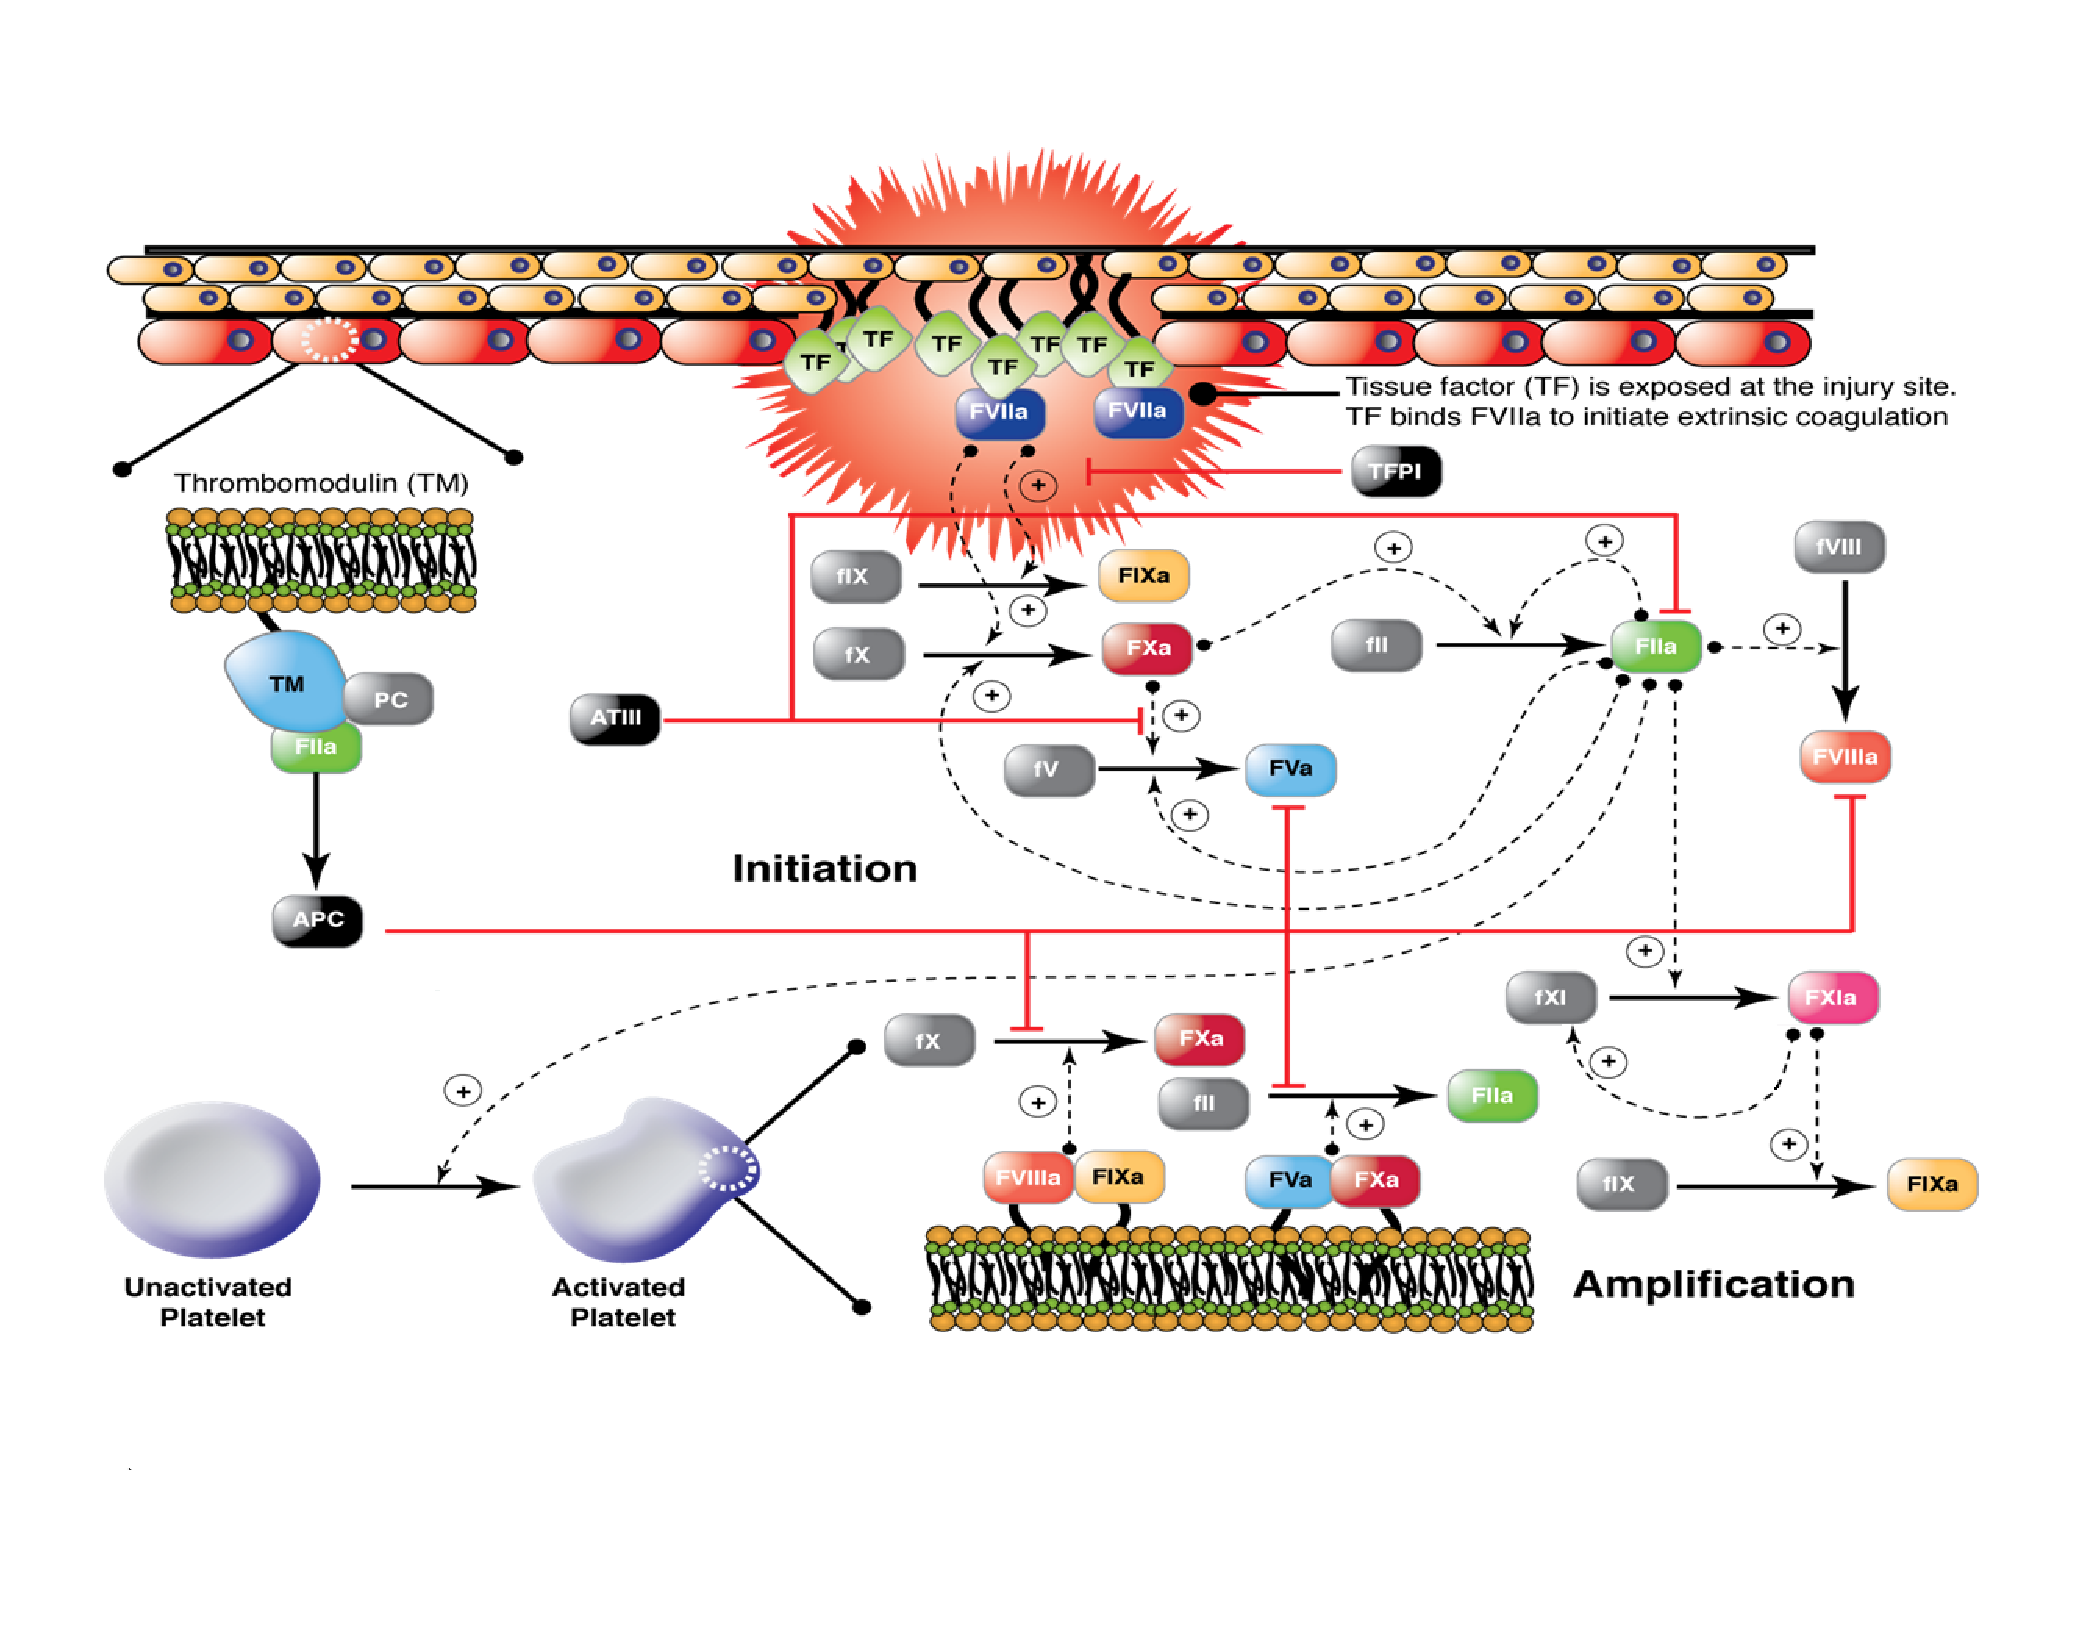
\includegraphics[width=1.00\textwidth,height=0.7\textheight]{./figs/Figure_2_CoagulationNetwork.pdf}
%\caption{Schematic of the extrinsic and intrinsic coagulation cascade. Inactive zymogens upstream (grey) are activated by exposure to tissue factor (TF) \cite{giesen1999blood} following vessel injury. Tissue factor and activated factor VIIa (FVIIa) form a complex that activates factor X (fX) and IX (fIX). FXa activates downstream factors including factor VIII (fVIII) and fIX. Factor V (fV) is primarily activated by thrombin (FIIa). In addition, we included a secondary fV activation route involving FXa. FXa and FVa form a complex (prothrombinase) on activated platelets that converts prothrombin (fII) to FIIa. FIXa and FVIIIa can also form a complex (tenase) on activated platelets which catalyzes FXa formation. Localized platelets are activated by external signals such as adenosine diphosphate (ADP) and thromboxane A2 (TXA2) or thrombin through protease-activated receptors (PARs) \protect\cite{coughlin2000thrombin} \protect \cite{coughlin1999protease} Thrombin also activates upstream coagulation factors, forming a strong positive feedback ensuring rapid activation. Tissue factor pathway inhibitor (TFPI) downregulates FXa formation and activity by sequestering free FXa and TF-FVIIa in a FXa-dependent manner. Antithrombin III (ATIII)  inhibits all proteases. Thrombin inhibits itself binding the surface protein thrombomodulin (TM) \protect\cite{esmon1989roles} The IIa-TM complex catalyzes the conversion of protein C (PC) to activated protein C (APC), which attenuates the coagulation response by the proteolytic cleavage of fV/FVa and fVIII/FVIIIa \protect\cite{esmon1989roles}}\label{fig-network}
%\end{figure}

\section*{Acknowledgements}
This study was supported by an award from the Army Research Office (ARO \#59155-LS).
\clearpage

%\bibliography{References_v1}
%\begin{thebibliography}{9999}
\bibliography{References_v2}

\clearpage

\begin{table}[h]
\centering
\caption{Error Analysis.}
\label{table:Error-Analysis}
\begin{center}
\begin{tabular}{ |c|c|c|c| } 
\hline
Simulation&Concentration& Standard Error & R-Squared Value \\
\hline
\multirow{3}{4em}{FVIIa-TF level} & 5nM & 0.0367 & 0.7680\\ 
& 500pM & 0.0636 & 0.8939\\
& 50pM & 0.1204 & 0.8384\\ 
& 10pM & 0.0813 & 0.9492\\
& 5pM & 0.0574 & 0.9794\\ 
\hline
\end{tabular}
\end{center}
\end{table}


\begin{table}[h]
\centering
\caption{Table with optimization settings and results for coagulation and different benchmarks using DdPSO.}
\label{table:benchmark-problems}
\resizebox{\columnwidth}{!}{
\begin{tabular}{|cccccc|}
\hline
                        & Coagulation           & \multicolumn{4}{l}{Benchmarks}\\
 \hline
                        & Experimental Data Set & B1           & B4          & Ackley 300D & Rastrigin 300D \\
 \hline
Lower Bound             & 0.001.pnom            & 5.pnom       & 5.pnom      & 30          & 5.12           \\
Upper Bound             & 1000.pnom             & 0.2.pnom     & 0.2.pnom    & -15         & -5.12          \\
CPU Time                & 10.0835 hours         & 38.308 hours & 6.2 minutes & 2.8 seconds & 2.6 seconds    \\
Function Evaluations    & 4000                  & 4000         & 4000        & 4000        & 4000           \\
Initial Objective Value & 1.11837e+07           & 1.4275e+07   & 1.8536e+07  & 21.12       & 99.985         \\
Final Objective Value   & 90456.9               & 4.96e+05     & 38.9375     & 0           & 0              \\
Nominal Objective Value & 4.7785e+06            & 1.0986e+06   & 39.0676     & 0           & 0      \\
\hline
\end{tabular}
}
\end{table}

\clearpage

\begin{figure}[h]
\centering
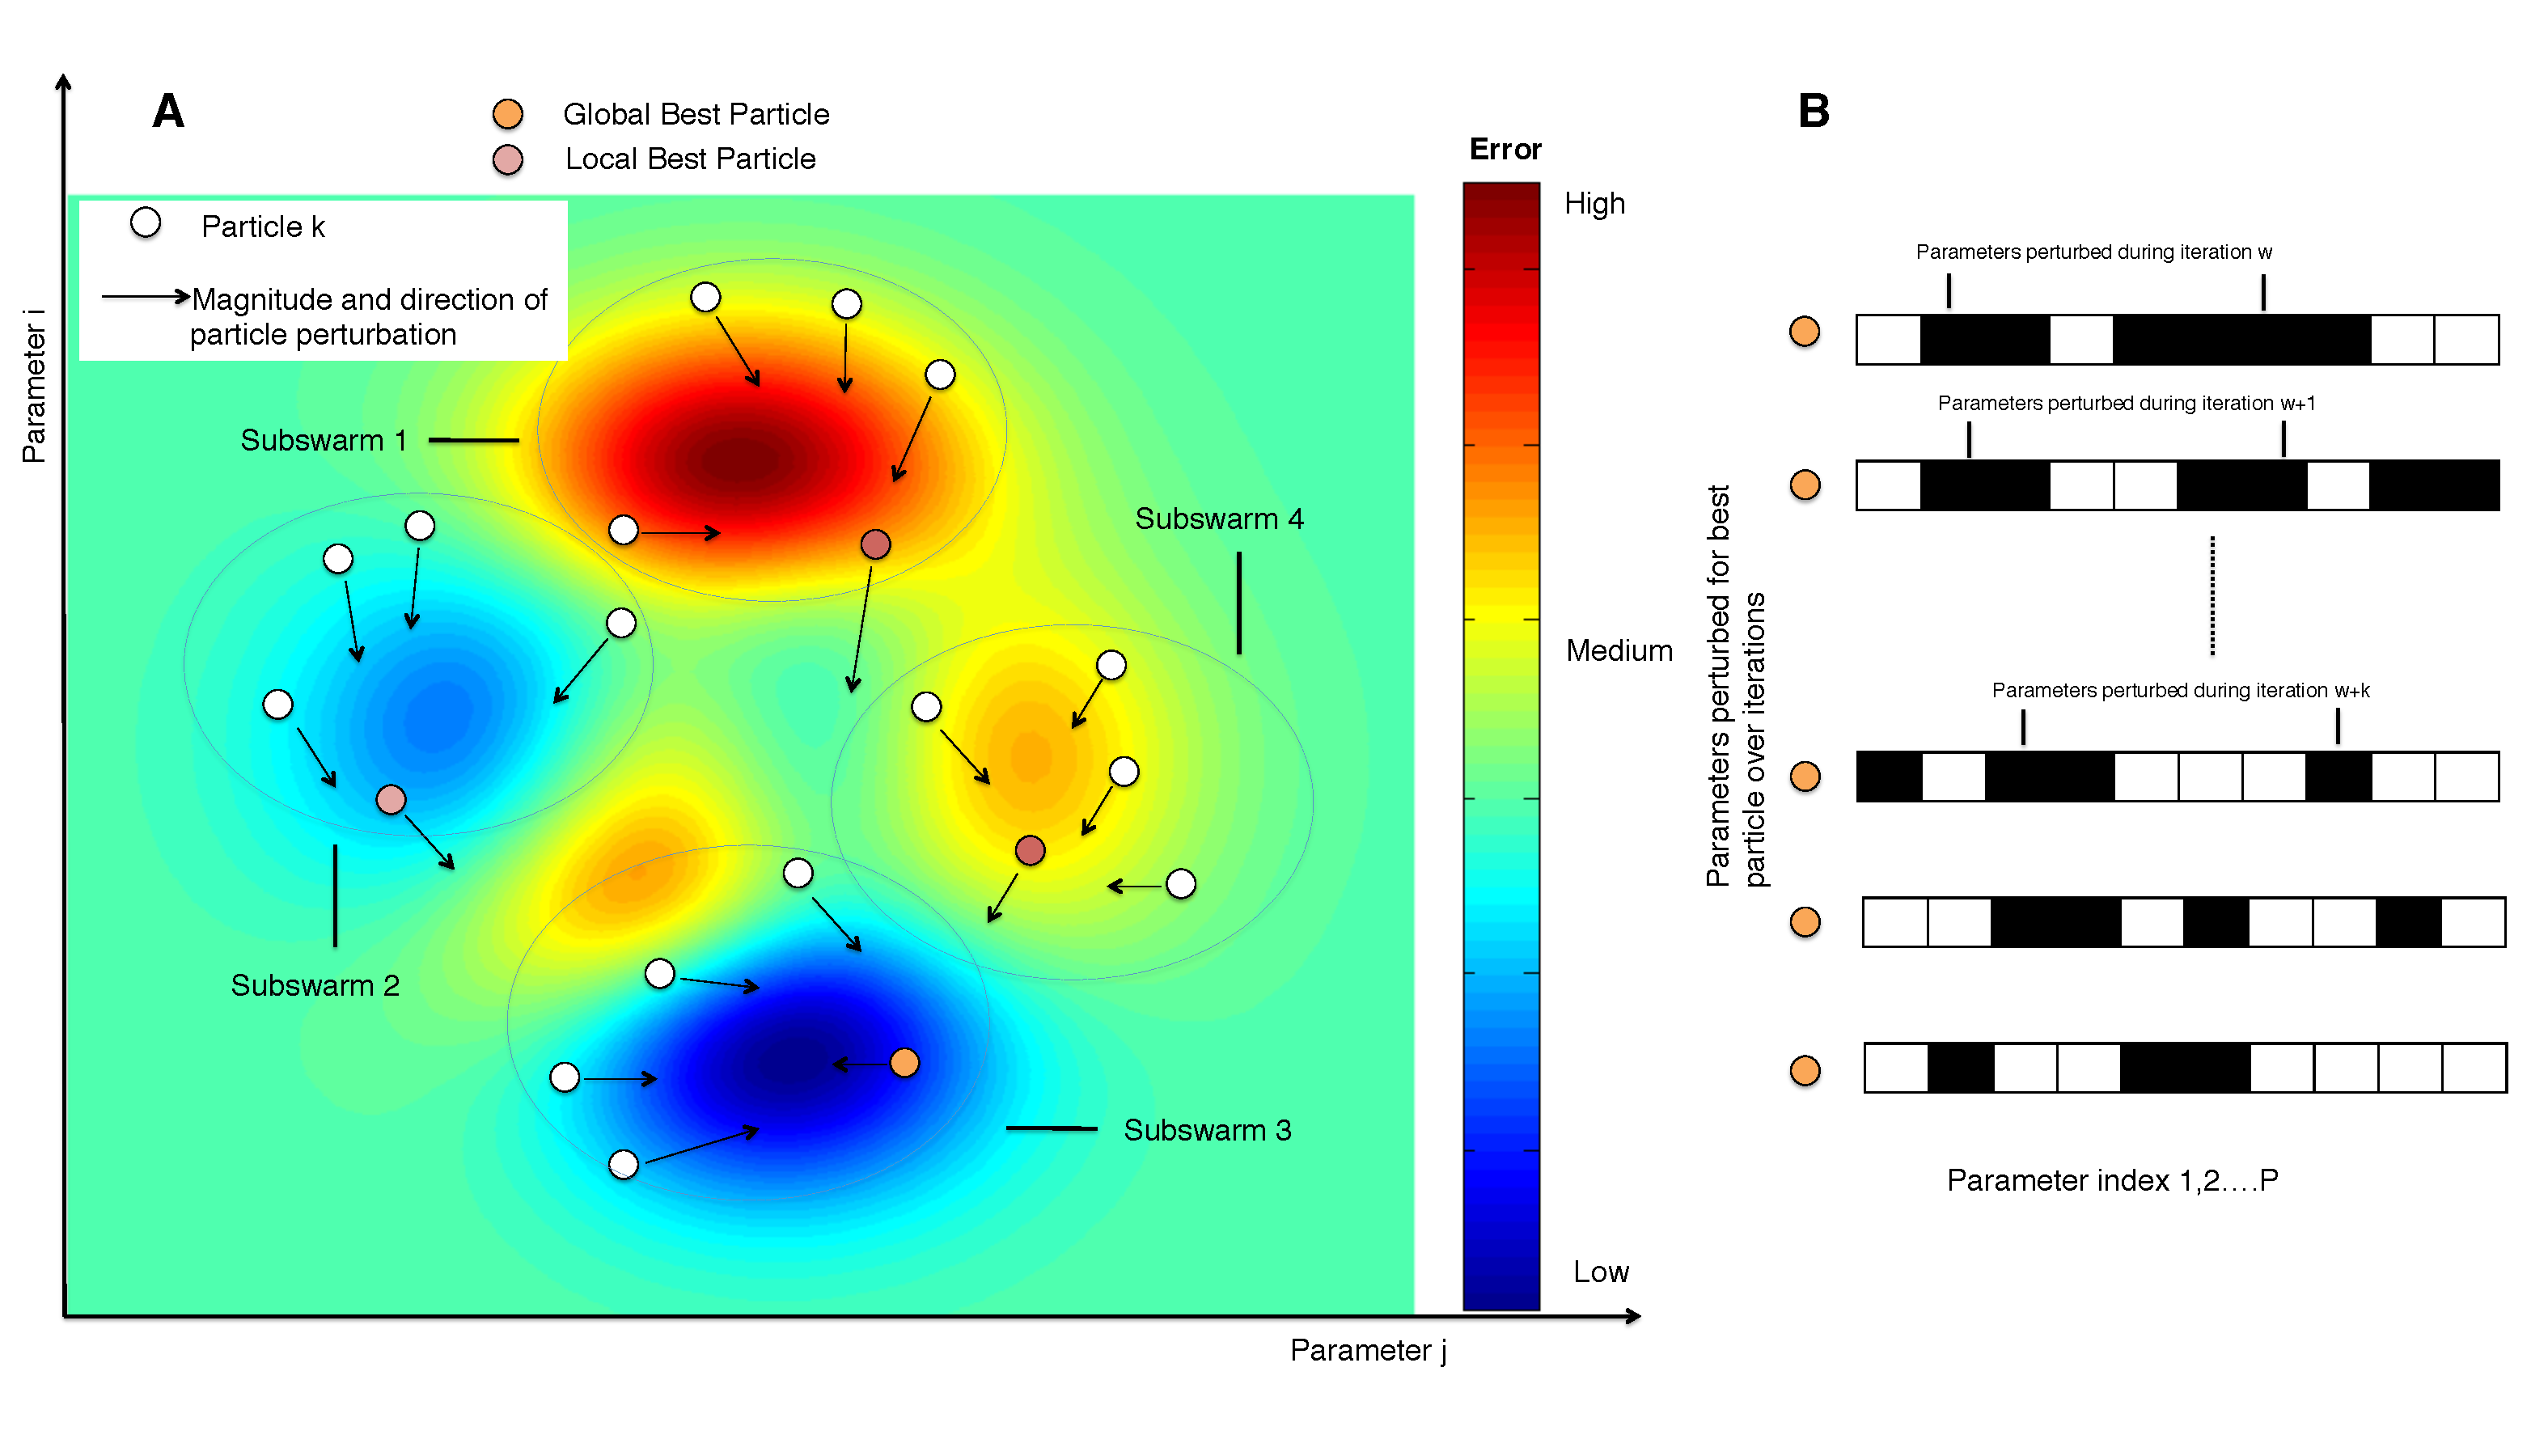
\includegraphics[width=1.0\textwidth,height=0.5\textheight]{./figs/Figure_1_Algorithm.pdf}
\caption{Multi Swarm Particle Swarm Optimization with Dynamically Dimensioned Search. \textbf{A}: Each particle represents an N dimensional parameter vector. Particles are randomly initialized and grouped into different sub-swarms. Within each swarm the magnitude and direction of the movement a particle is influenced by the position of the best particle and also by its own experience. After every $\mathbf{g}$ number of function evaluations the particles are mixed and randomly assigned to different swarms. At the end of the evaluations ($\mathcal{FR}$) assigned to swarm search, the global best particle (orange color) amongst all sub-swarms is chosen as the candidate parameter vector for Dynamically Dimensioned Search \textbf{B}: The candidate vector does a greedy search in a dynamic neighborhood. The search neighborhood is dynamically adjusted by varying the number of dimensions that are perturbed (in black) in each evaluation step. The probability that a dimension is perturbed decreases as the number of function evaluations increase. Thus as the evaluations increase the optimality of the solution is preserved.
}\label{fig-algorithm}
\end{figure}

\clearpage

\begin{figure}[h]
\centering
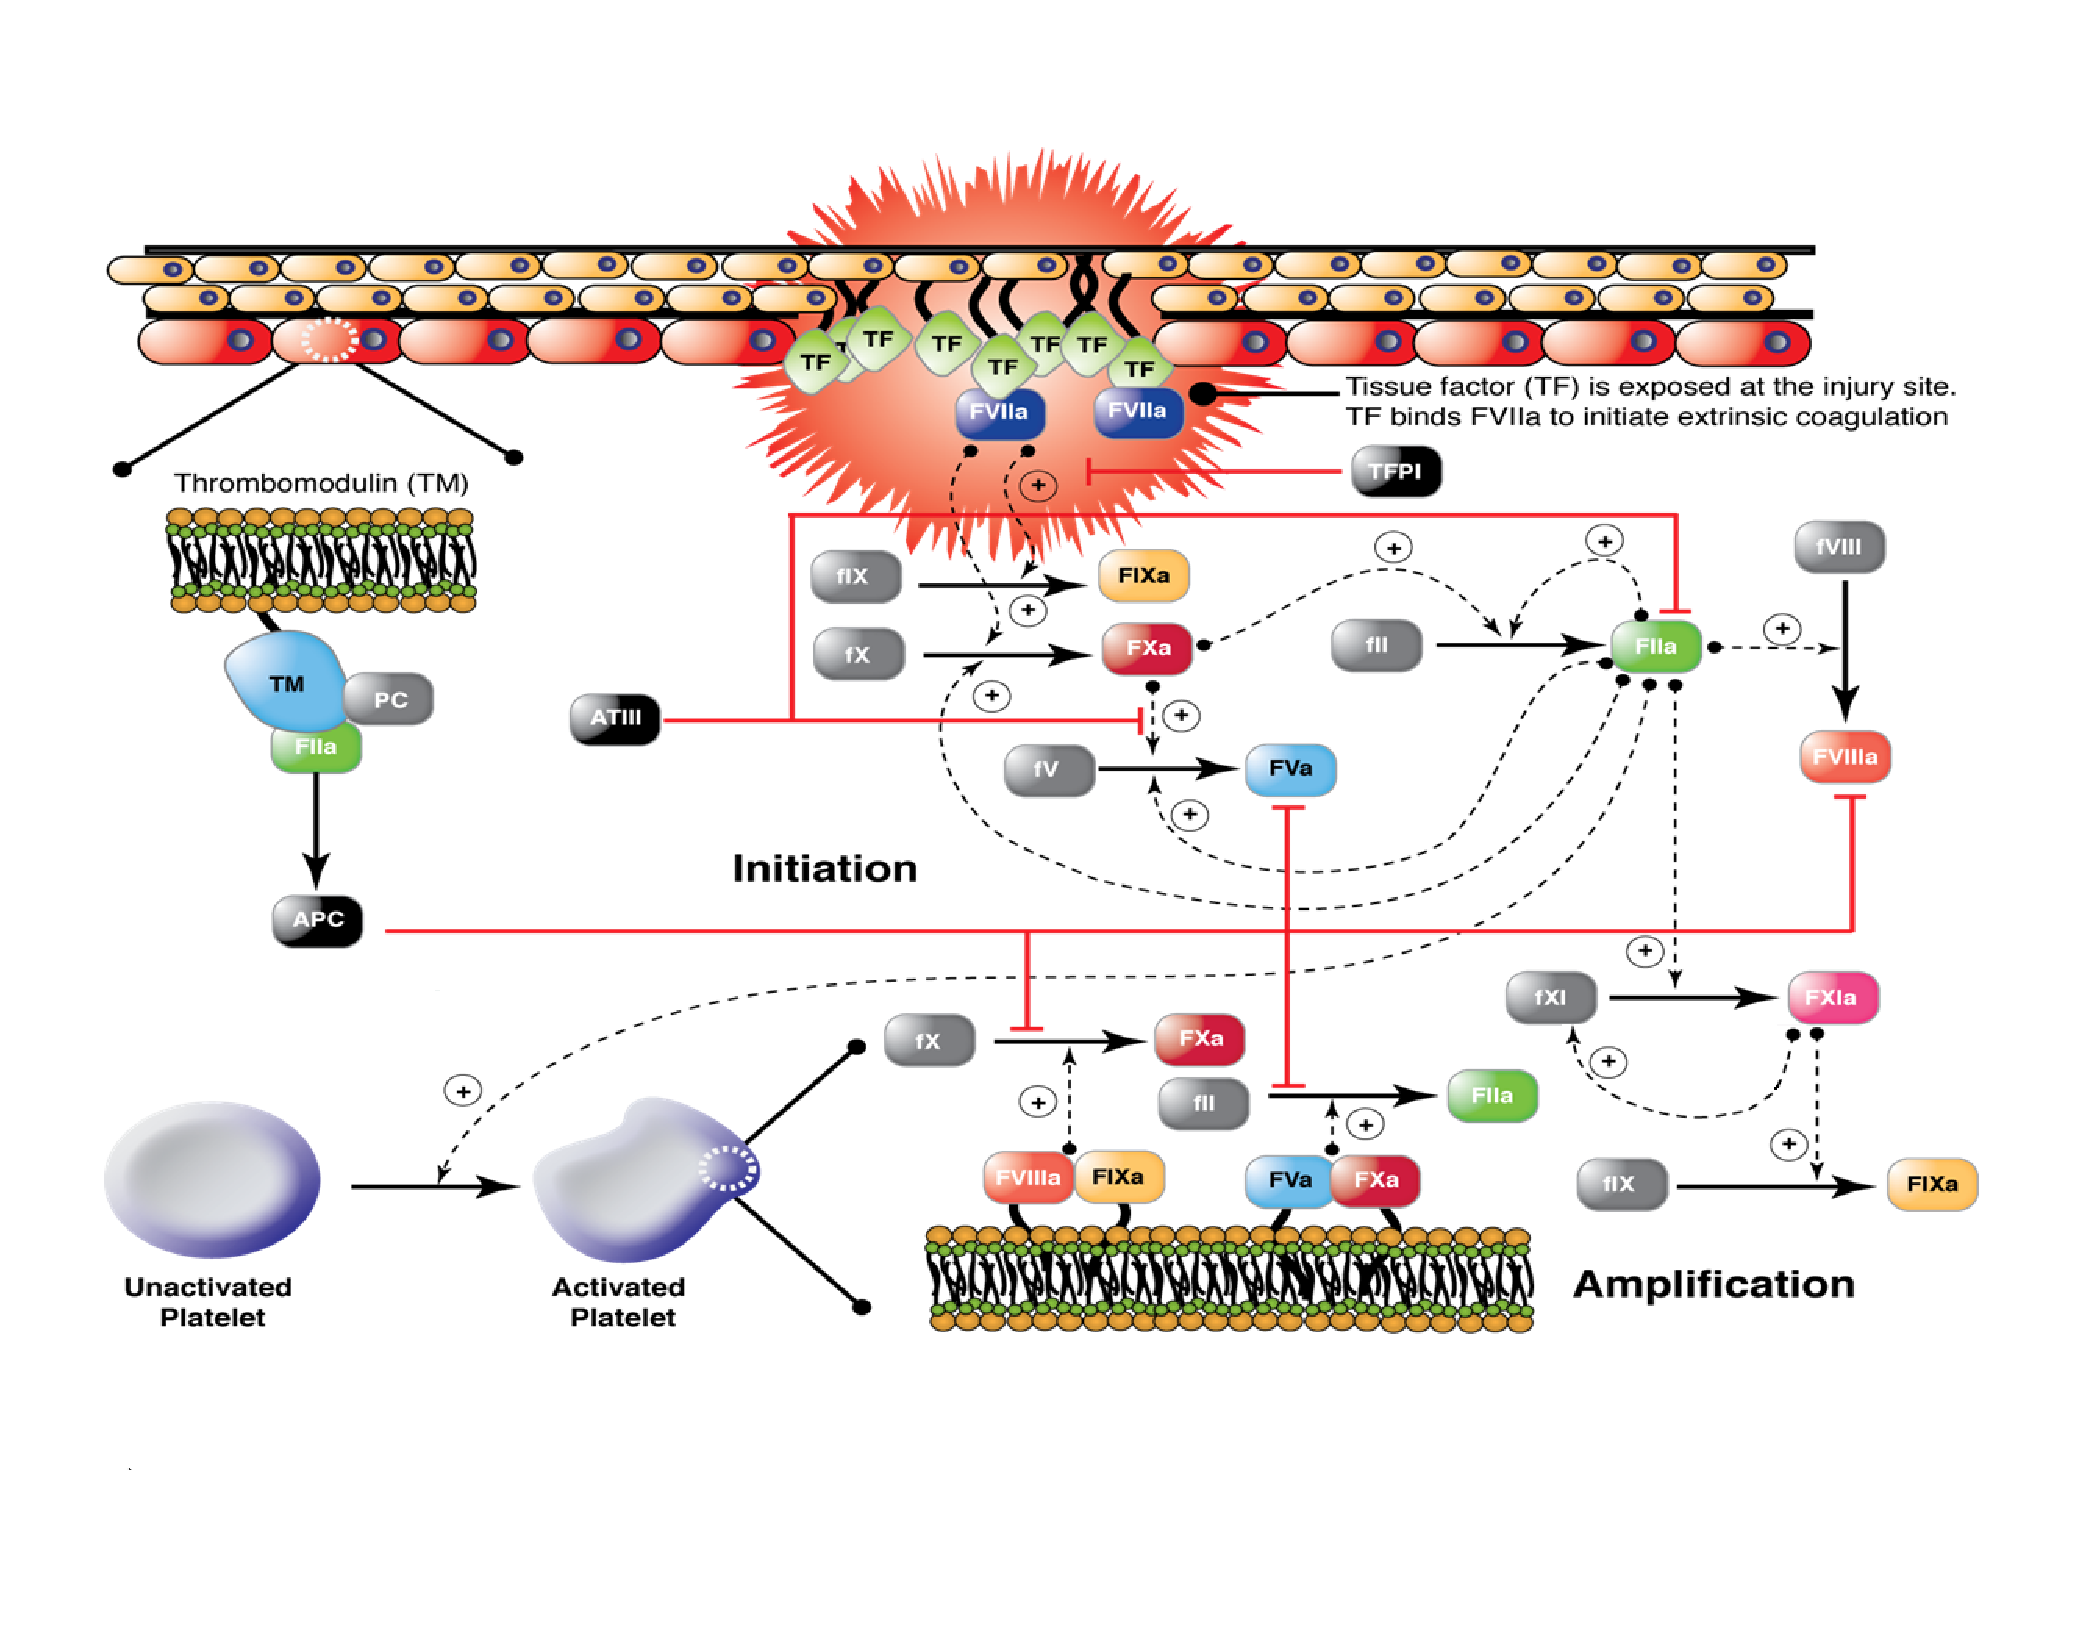
\includegraphics[width=1.00\textwidth,height=0.7\textheight]{./figs/Figure_2_CoagulationNetwork.pdf}
\caption{Schematic of the extrinsic and intrinsic coagulation cascade. Inactive zymogens upstream (grey) are activated by exposure to tissue factor (TF)  following vessel injury. Tissue factor and activated factor VIIa (FVIIa) form a complex that activates factor X (fX) and IX (fIX). FXa activates downstream factors including factor VIII (fVIII) and fIX. Factor V (fV) is primarily activated by thrombin (FIIa). In addition, we included a secondary fV activation route involving FXa. FXa and FVa form a complex (prothrombinase) on activated platelets that converts prothrombin (fII) to FIIa. FIXa and FVIIIa can also form a complex (tenase) on activated platelets which catalyzes FXa formation.  Thrombin also activates upstream coagulation factors, forming a strong positive feedback ensuring rapid activation. Tissue factor pathway inhibitor (TFPI) downregulates FXa formation and activity by sequestering free FXa and TF-FVIIa in a FXa-dependent manner. Antithrombin III (ATIII)  inhibits all proteases. Thrombin inhibits itself binding the surface protein thrombomodulin (TM). The IIa-TM complex catalyzes the conversion of protein C (PC) to activated protein C (APC), which attenuates the coagulation response by the proteolytic cleavage of fV/FVa and fVIII/FVIIIa. }\label{fig-coagulation-network}
\end{figure}

\clearpage

\begin{figure}[h]
\centering
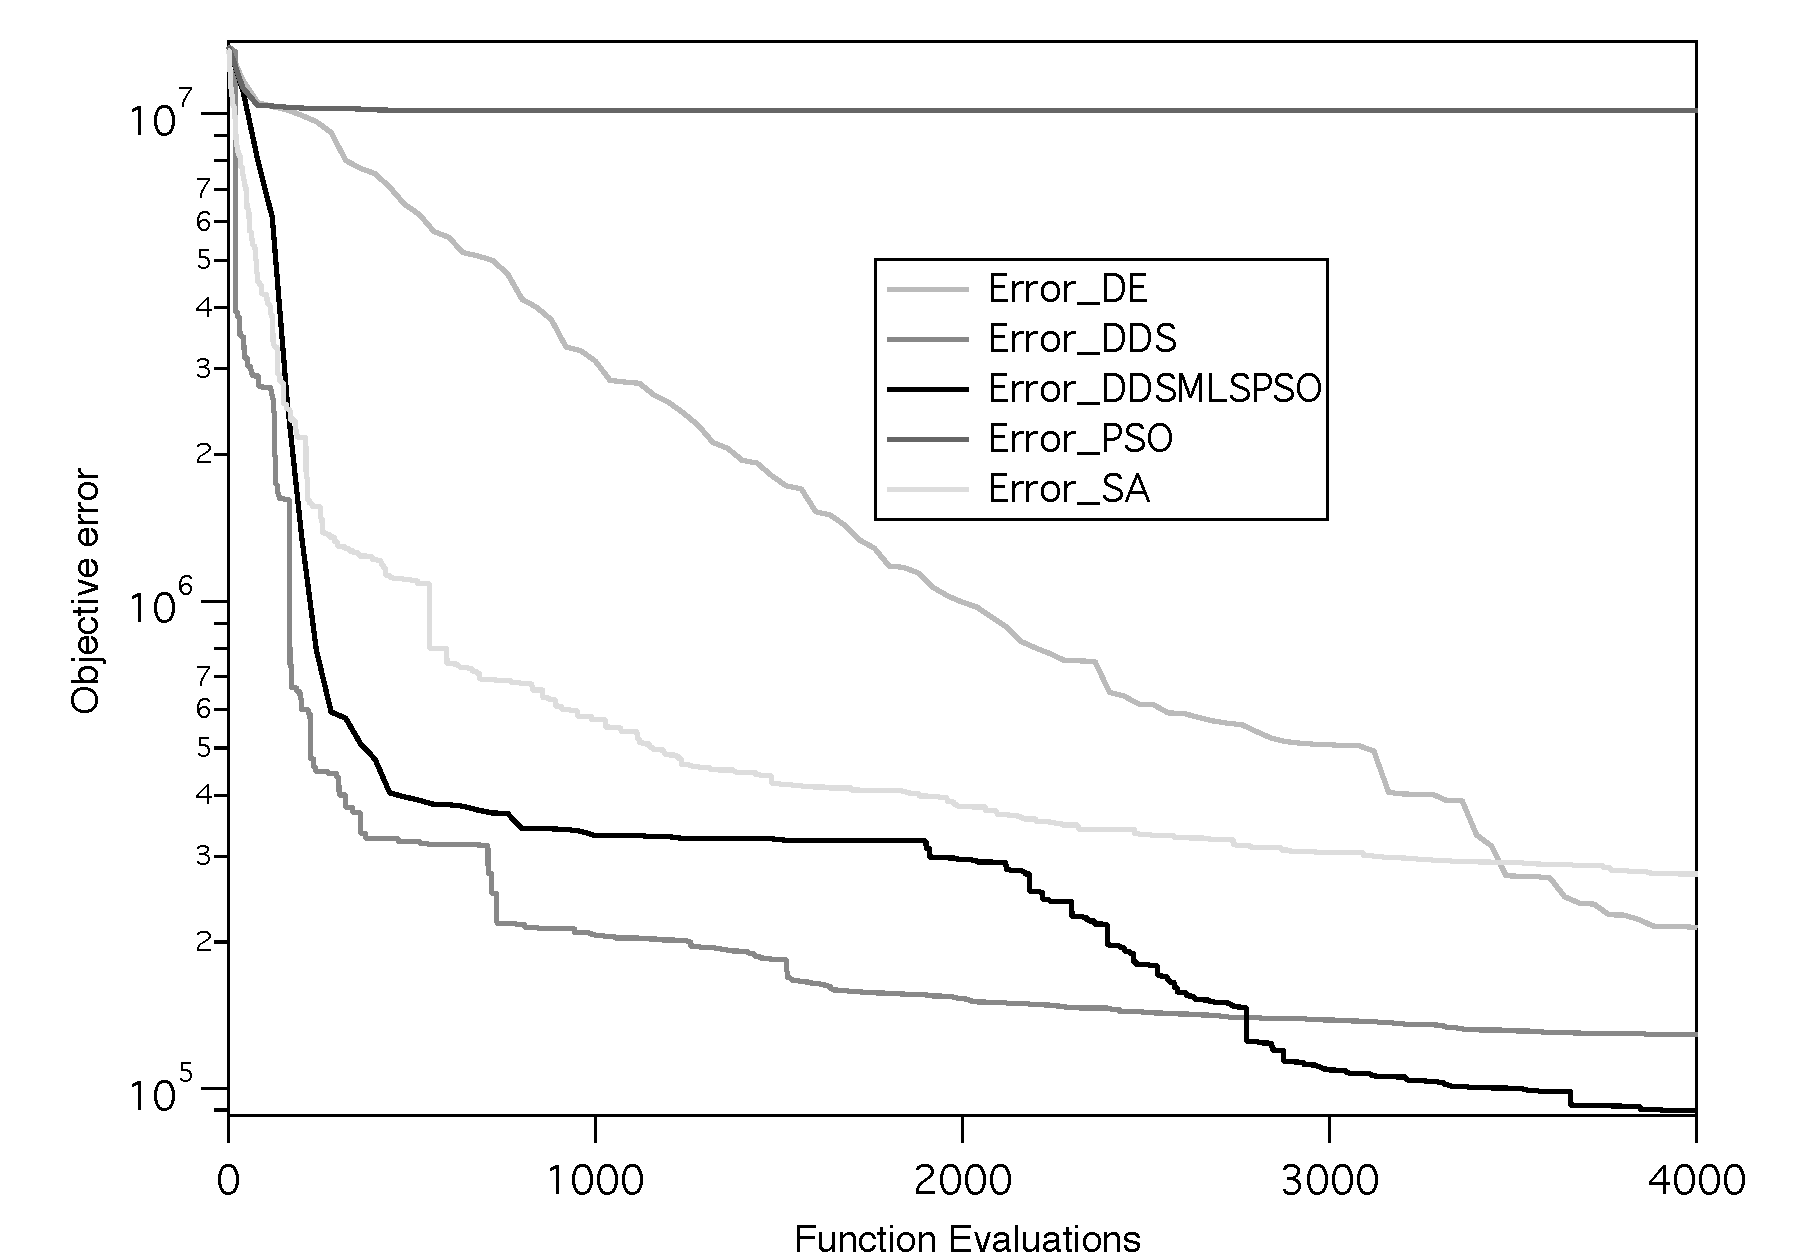
\includegraphics[width=1.0\textwidth,height=0.5\textheight]{./figs/Figure_3_Errors_convergence.pdf}
\caption{Error convergence rates of the 5 different algorithms on the coagulation model. The objective error is the mean over $N$= 25 trials. DDSMLSPSO and DDS have the steepest drop in error during first 2000 function evaluations. Thereafter the error drop in DDS remains nearly constant whereas DDSMLSPSO drops further from around 2000 to 4000 function evaluations. At the end of 4000 function evaluations DDSMLSPSO attains the lowest error.
}\label{fig-train}
\end{figure}

\clearpage

\begin{figure}[h]
\centering
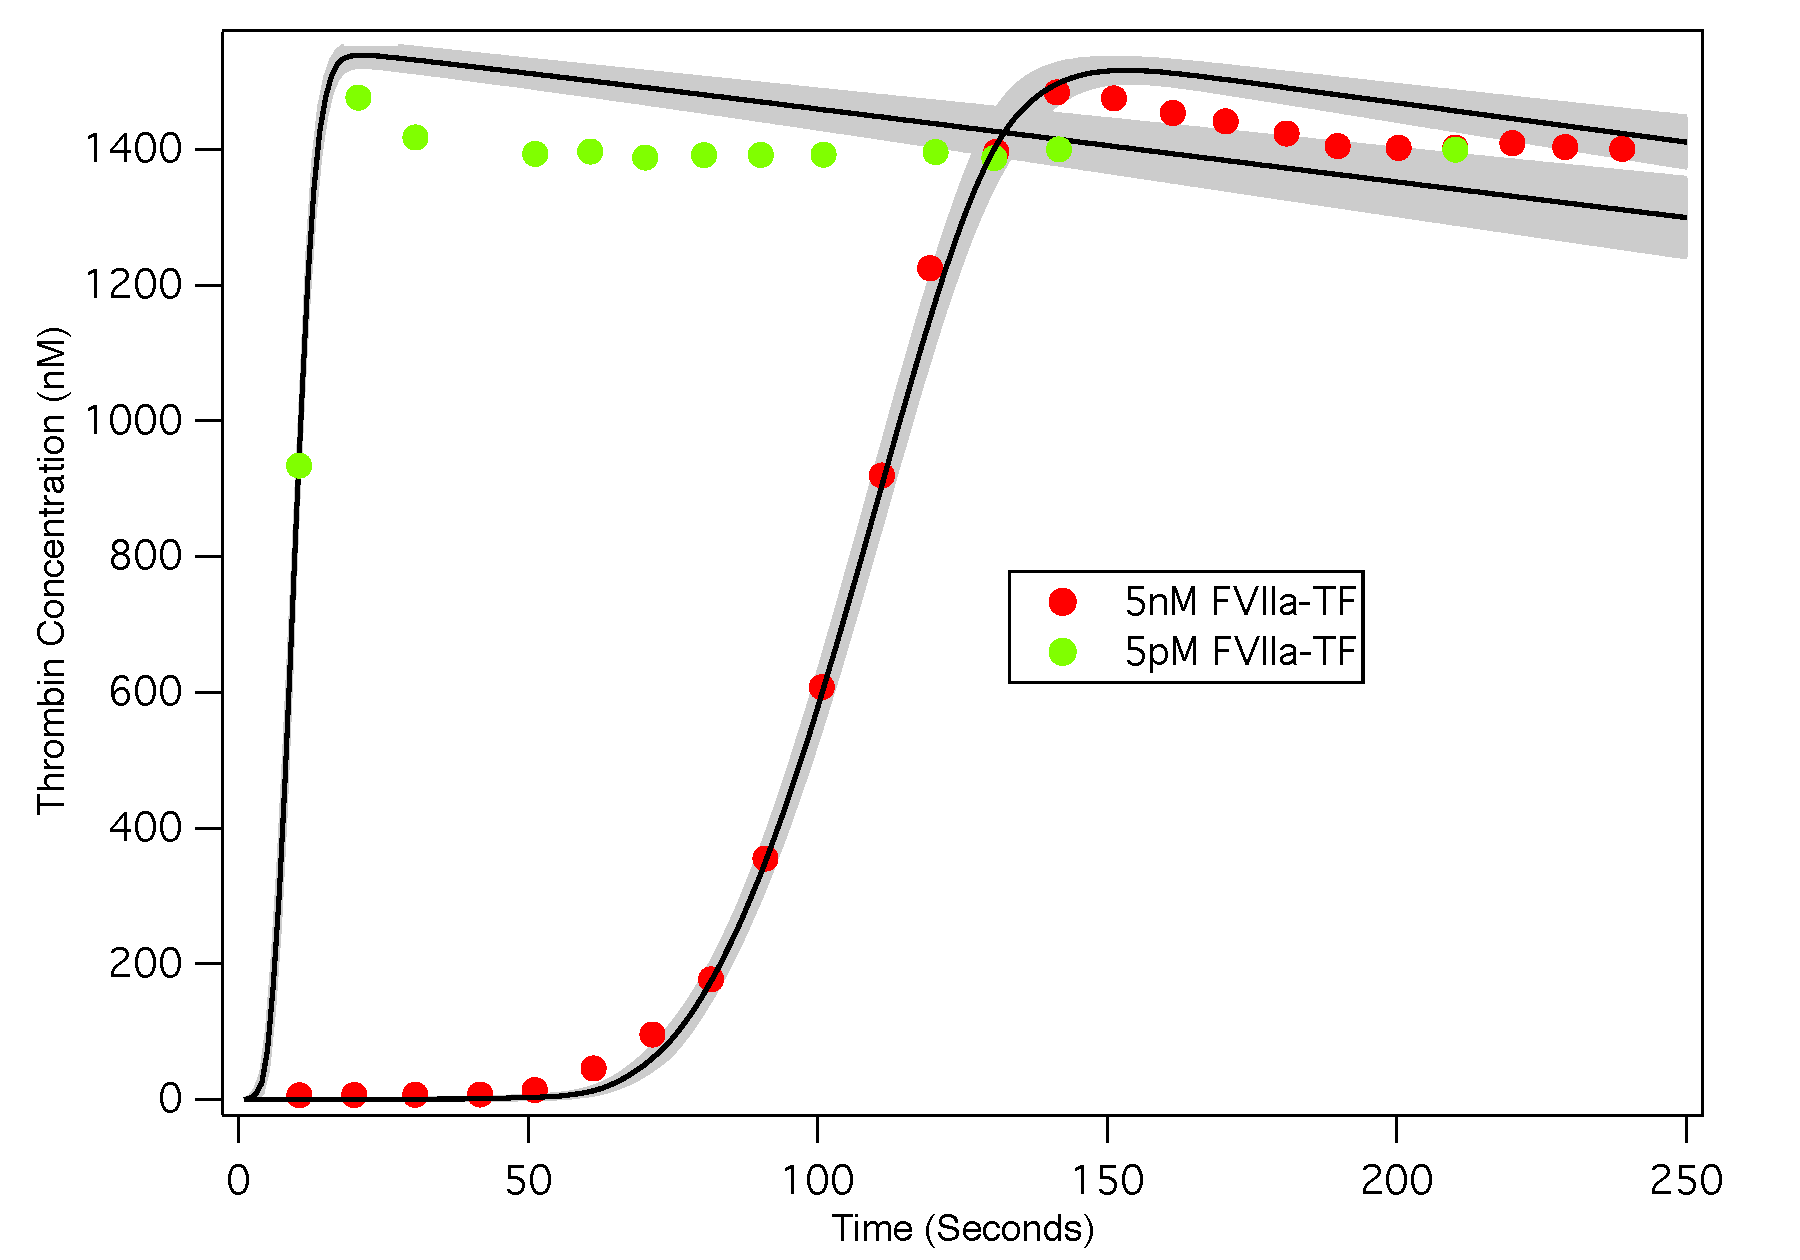
\includegraphics[width=1.0\textwidth,height=0.5\textheight]{./figs/Figure_4_Sim_Train_E1_E5.pdf}
\caption{Model fits on experimental data using DDSMLSPSO. The model parameters were estimated using DDSMLSPSO. Solid black lines indicate the simulated mean thrombin concentration using parameter vectors from $N$= 25 trials. The grey shaded region represents the 99\% confidence estimate of the mean simulated thrombin concentration. The experimental data is reproduced from the synthetic plasma assays of Mann and co-workers. Thrombin generation is initiated by adding Factor VIIa-TF (5nM - Red and 5pM - Green) to synthetic plasma containing 200 $\mu$mol/L of phospholipid vesicles (PCPS) and a mixture of coagulation factors (II,V,VII,VIII,IX,X and XI) at their mean plasma concentrations.
}\label{fig-train}
\end{figure}

\clearpage

\begin{figure}[h]
\centering
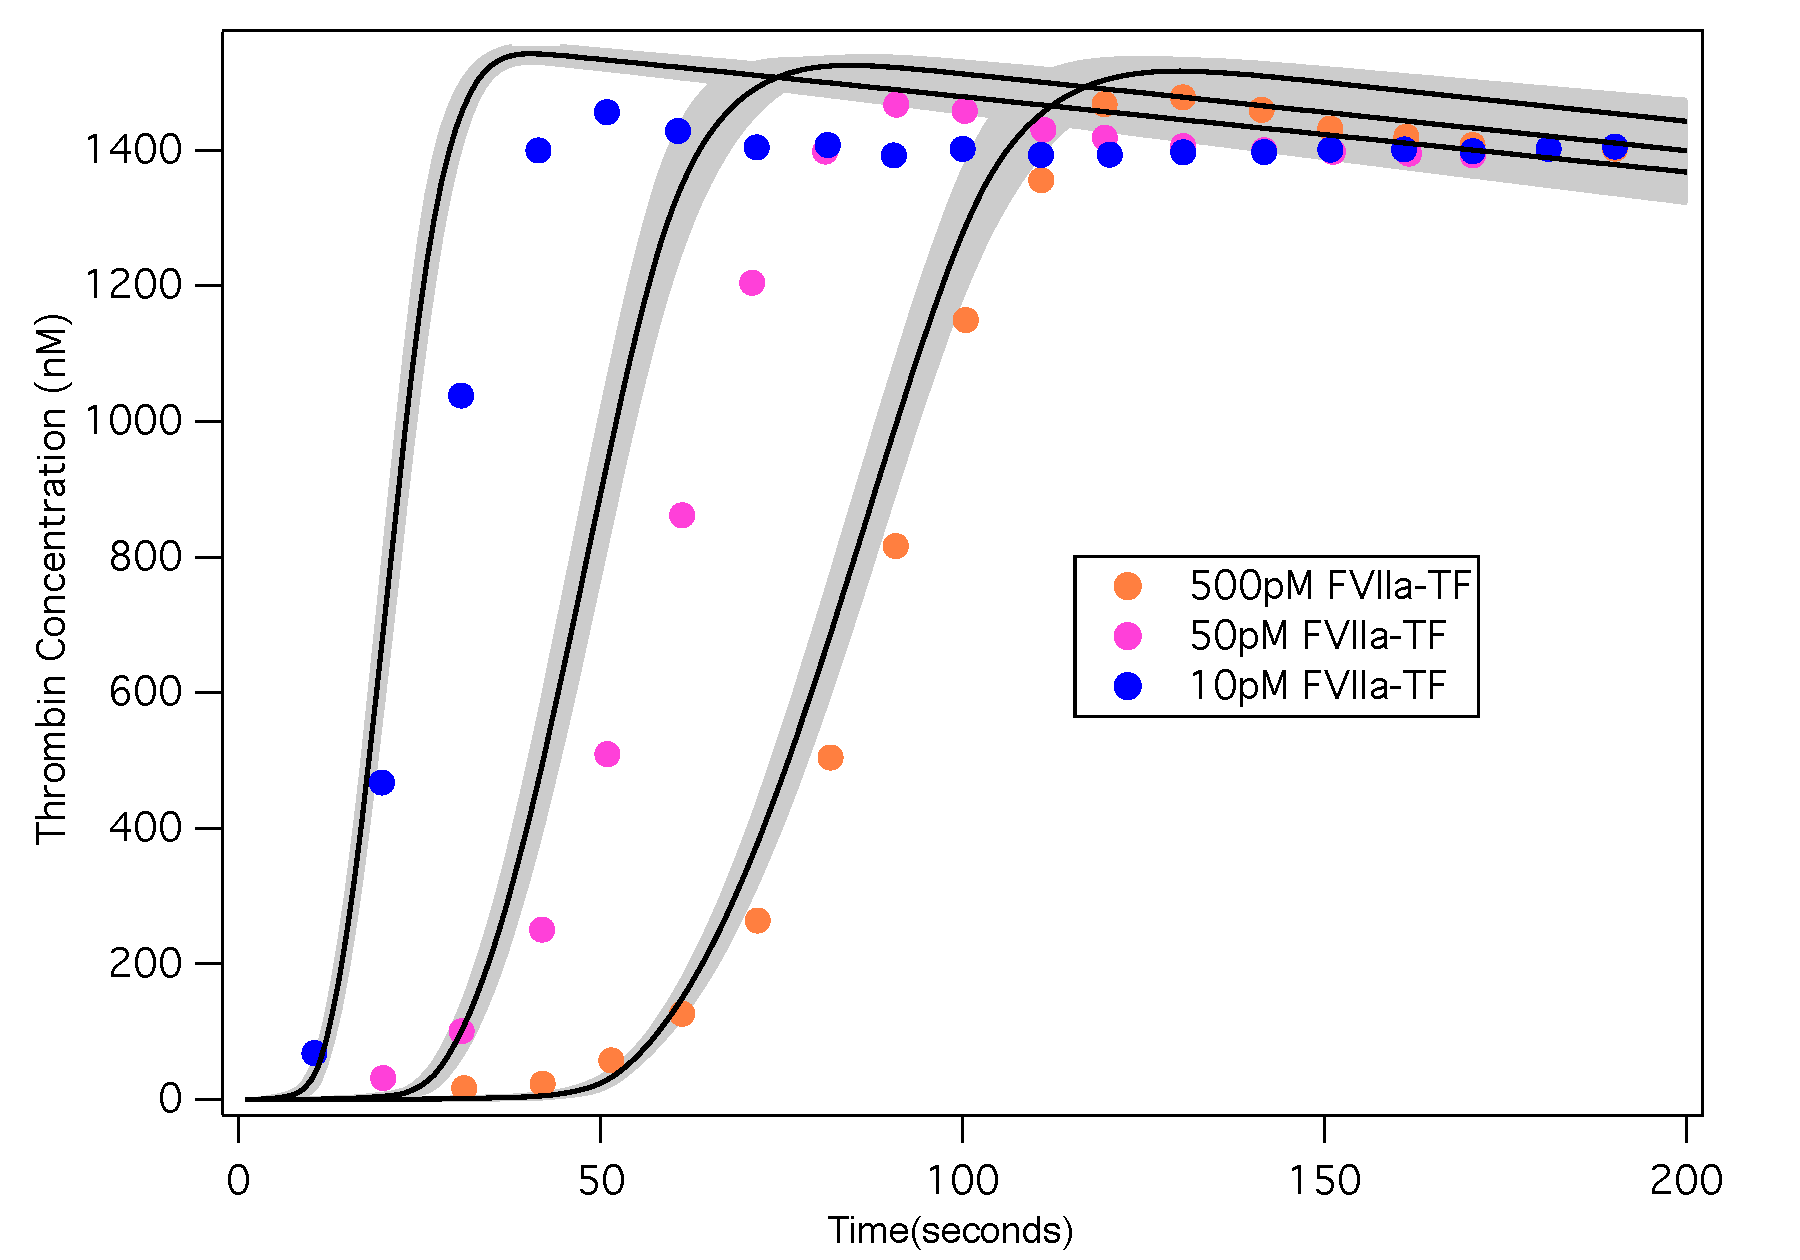
\includegraphics[width=1.0\textwidth,height=0.5\textheight]{./figs/Figure_5_Sim_Validate_E2_E4_E6.pdf}
\caption{Model predictions on unseen experimental data using parameters obtained from DDSMLSPSO. The parameter estimates that were obtained using DDSMLSPSO were tested against data that was not used in the model training. Solid black lines indicate the simulated mean thrombin concentration using parameter vectors from $N$= 25 trials. The grey shaded region represents the 99\% confidence estimate of the mean simulated thrombin concentration. The experimental data is reproduced from the synthetic plasma assays of Mann and co-workers. Thrombin generation is initiated by adding Factor VIIa-TF (500pM - Blue, 50pM - Pink and 10pM - Orange respectively) to synthetic plasma containing 200 $\mu$mol/L of phospholipid vesicles (PCPS) and a mixture of coagulation factors (II,V,VII,VIII,IX,X and XI) at their mean plasma concentrations.
}\label{fig-validation}
\end{figure}

%\bibitem[Saltelli \em{et~al.}(2010)Saltelli, Annoni, Azzini, Campolongo, Ratto,
  %and Tarantola]{Saltelli:2010}
%Saltelli, A.; Annoni, P.; Azzini, I.; Campolongo, F.; Ratto, M.; Tarantola, S.
%\newblock Variance based sensitivity analysis of model output. Design and
  %estimator for the total sensitivity index.
%\newblock {\em Comput. Phys. Commun.} {\bf 2010}, {\em 181},~259--270.

%\end{thebibliography}

\clearpage

% Supplemental figures -
% Set the S-
\renewcommand\thefigure{S\arabic{figure}}
\renewcommand\thetable{T\arabic{table}}
\renewcommand\thepage{S-\arabic{page}}
\renewcommand\theequation{S\arabic{equation}}

% Reset the counters -
\setcounter{equation}{0}
\setcounter{table}{0}
\setcounter{figure}{0}
\setcounter{page}{1}

\begin{figure}[ht]
\centering
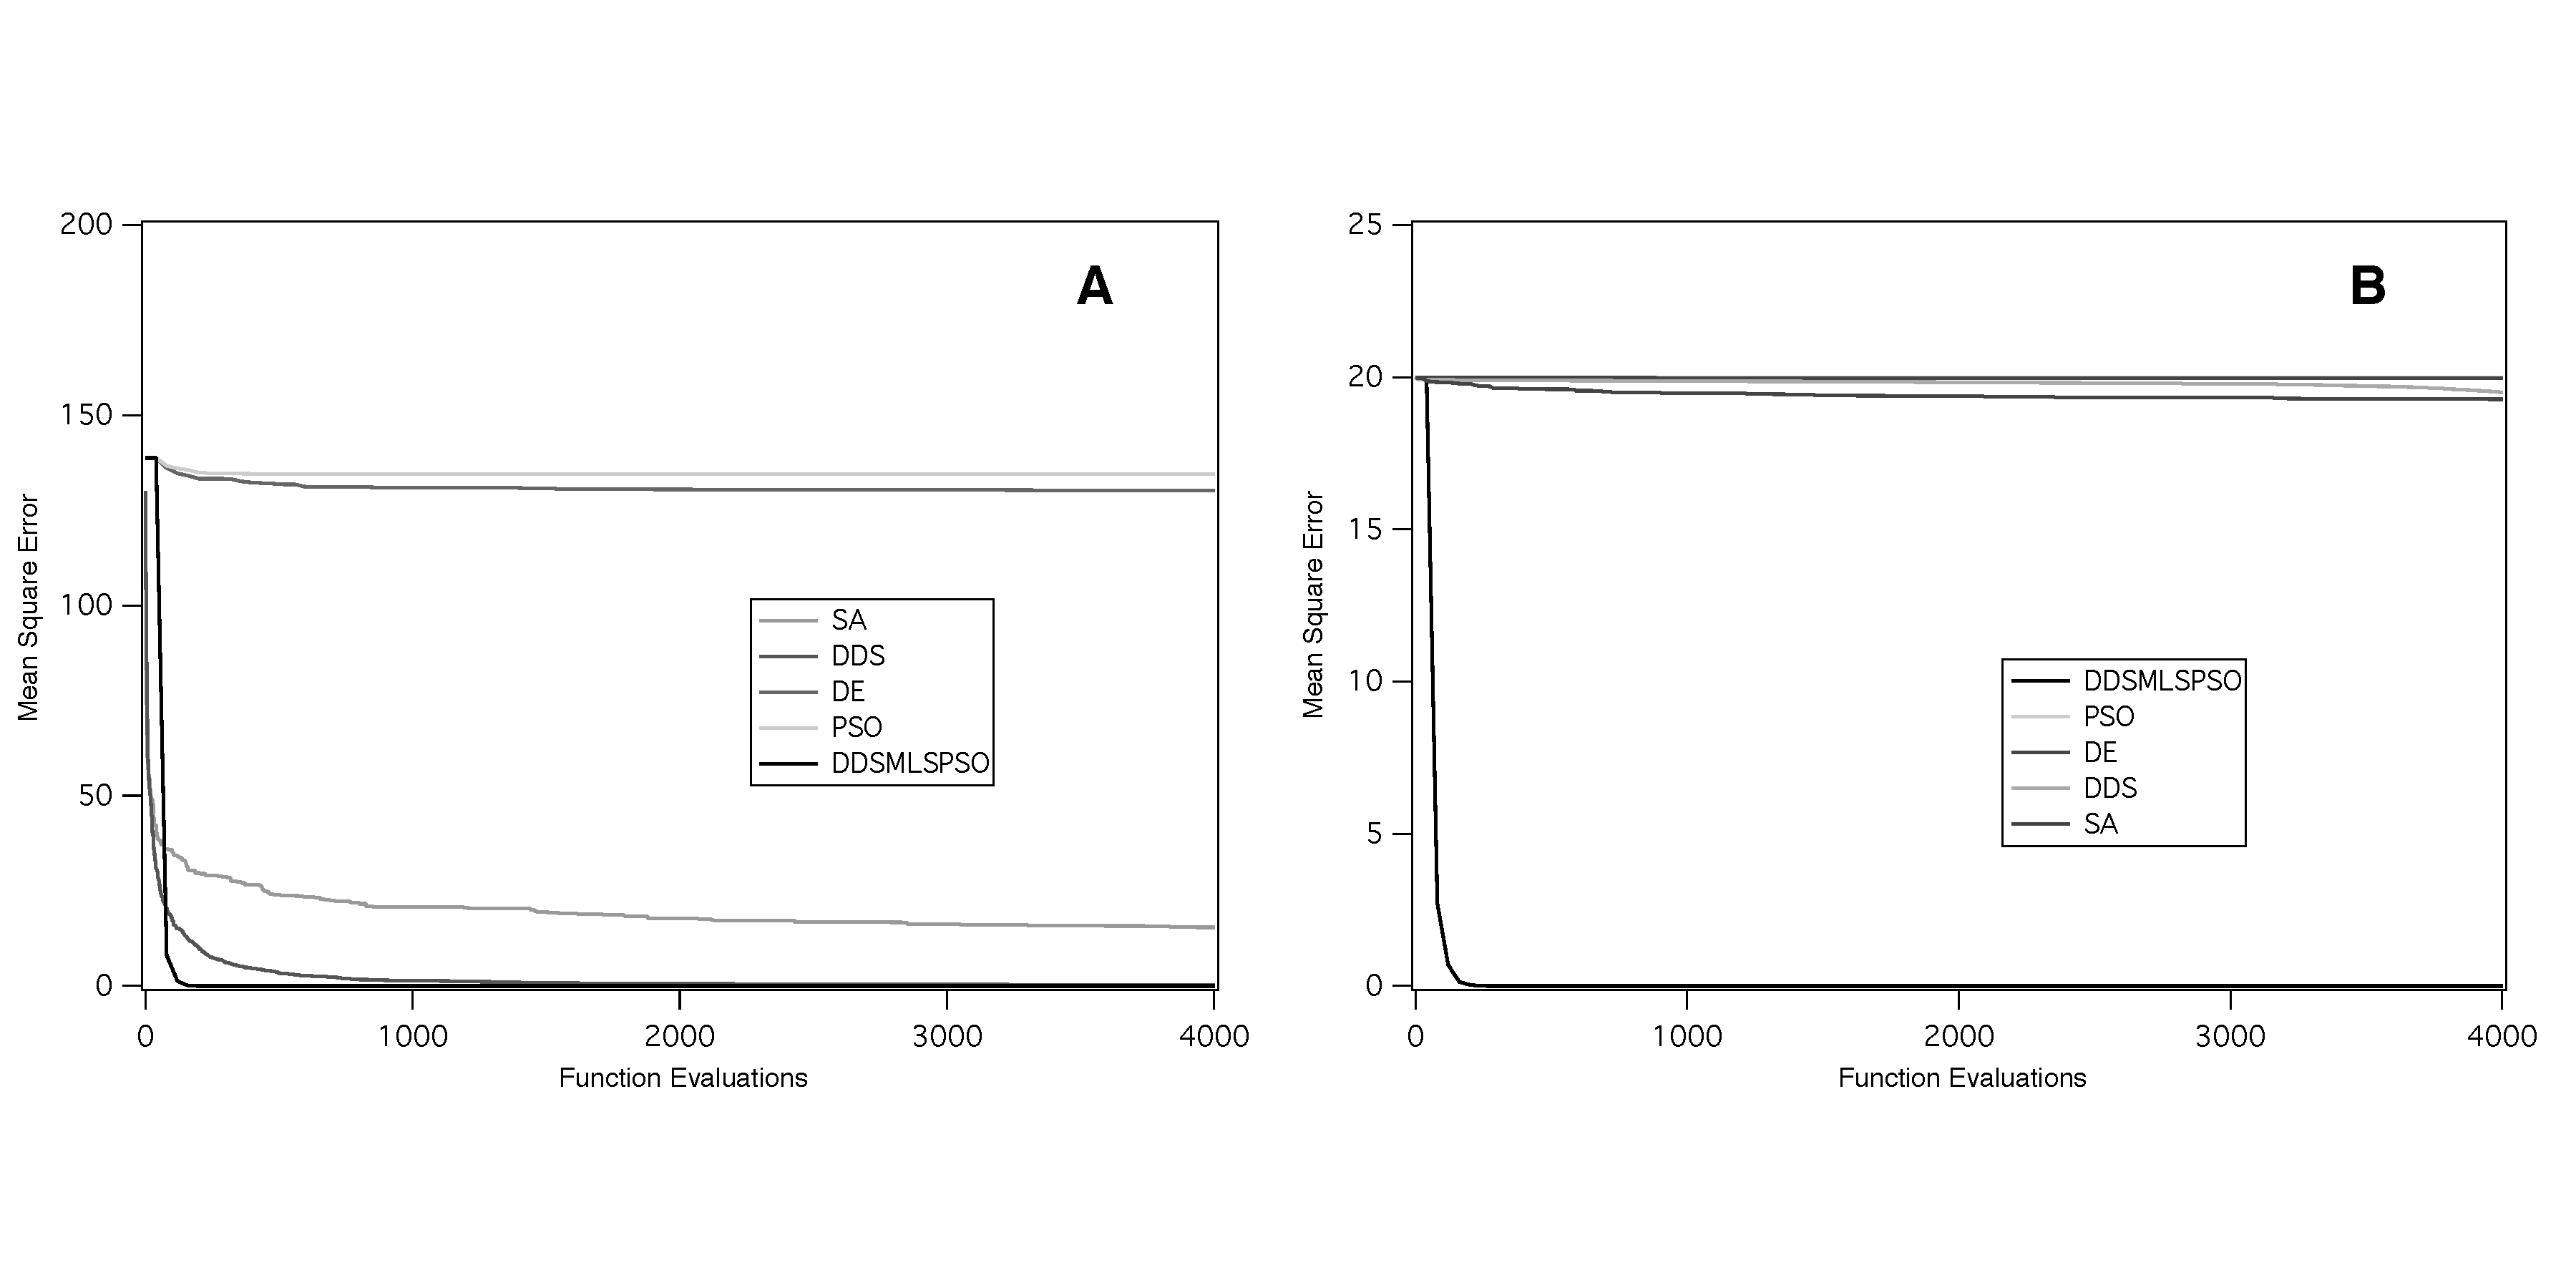
\includegraphics[width=1.02\textwidth,height=0.5\textheight]{./figs/Figure_6_Ackley_Rast}
\caption{Error convergence on 300 dimensional Ackley function and Rastrigin function. \textbf {(A)} Error convergence of 5 different meta-heuristics on 300 dimensional Ackley function \textbf {(B)} Error convergence of 5 different meta-heuristics on 300 dimensional Rastrigin function
}\label{fig-testfunctions}
\end{figure}



\begin{figure}[ht]
\centering
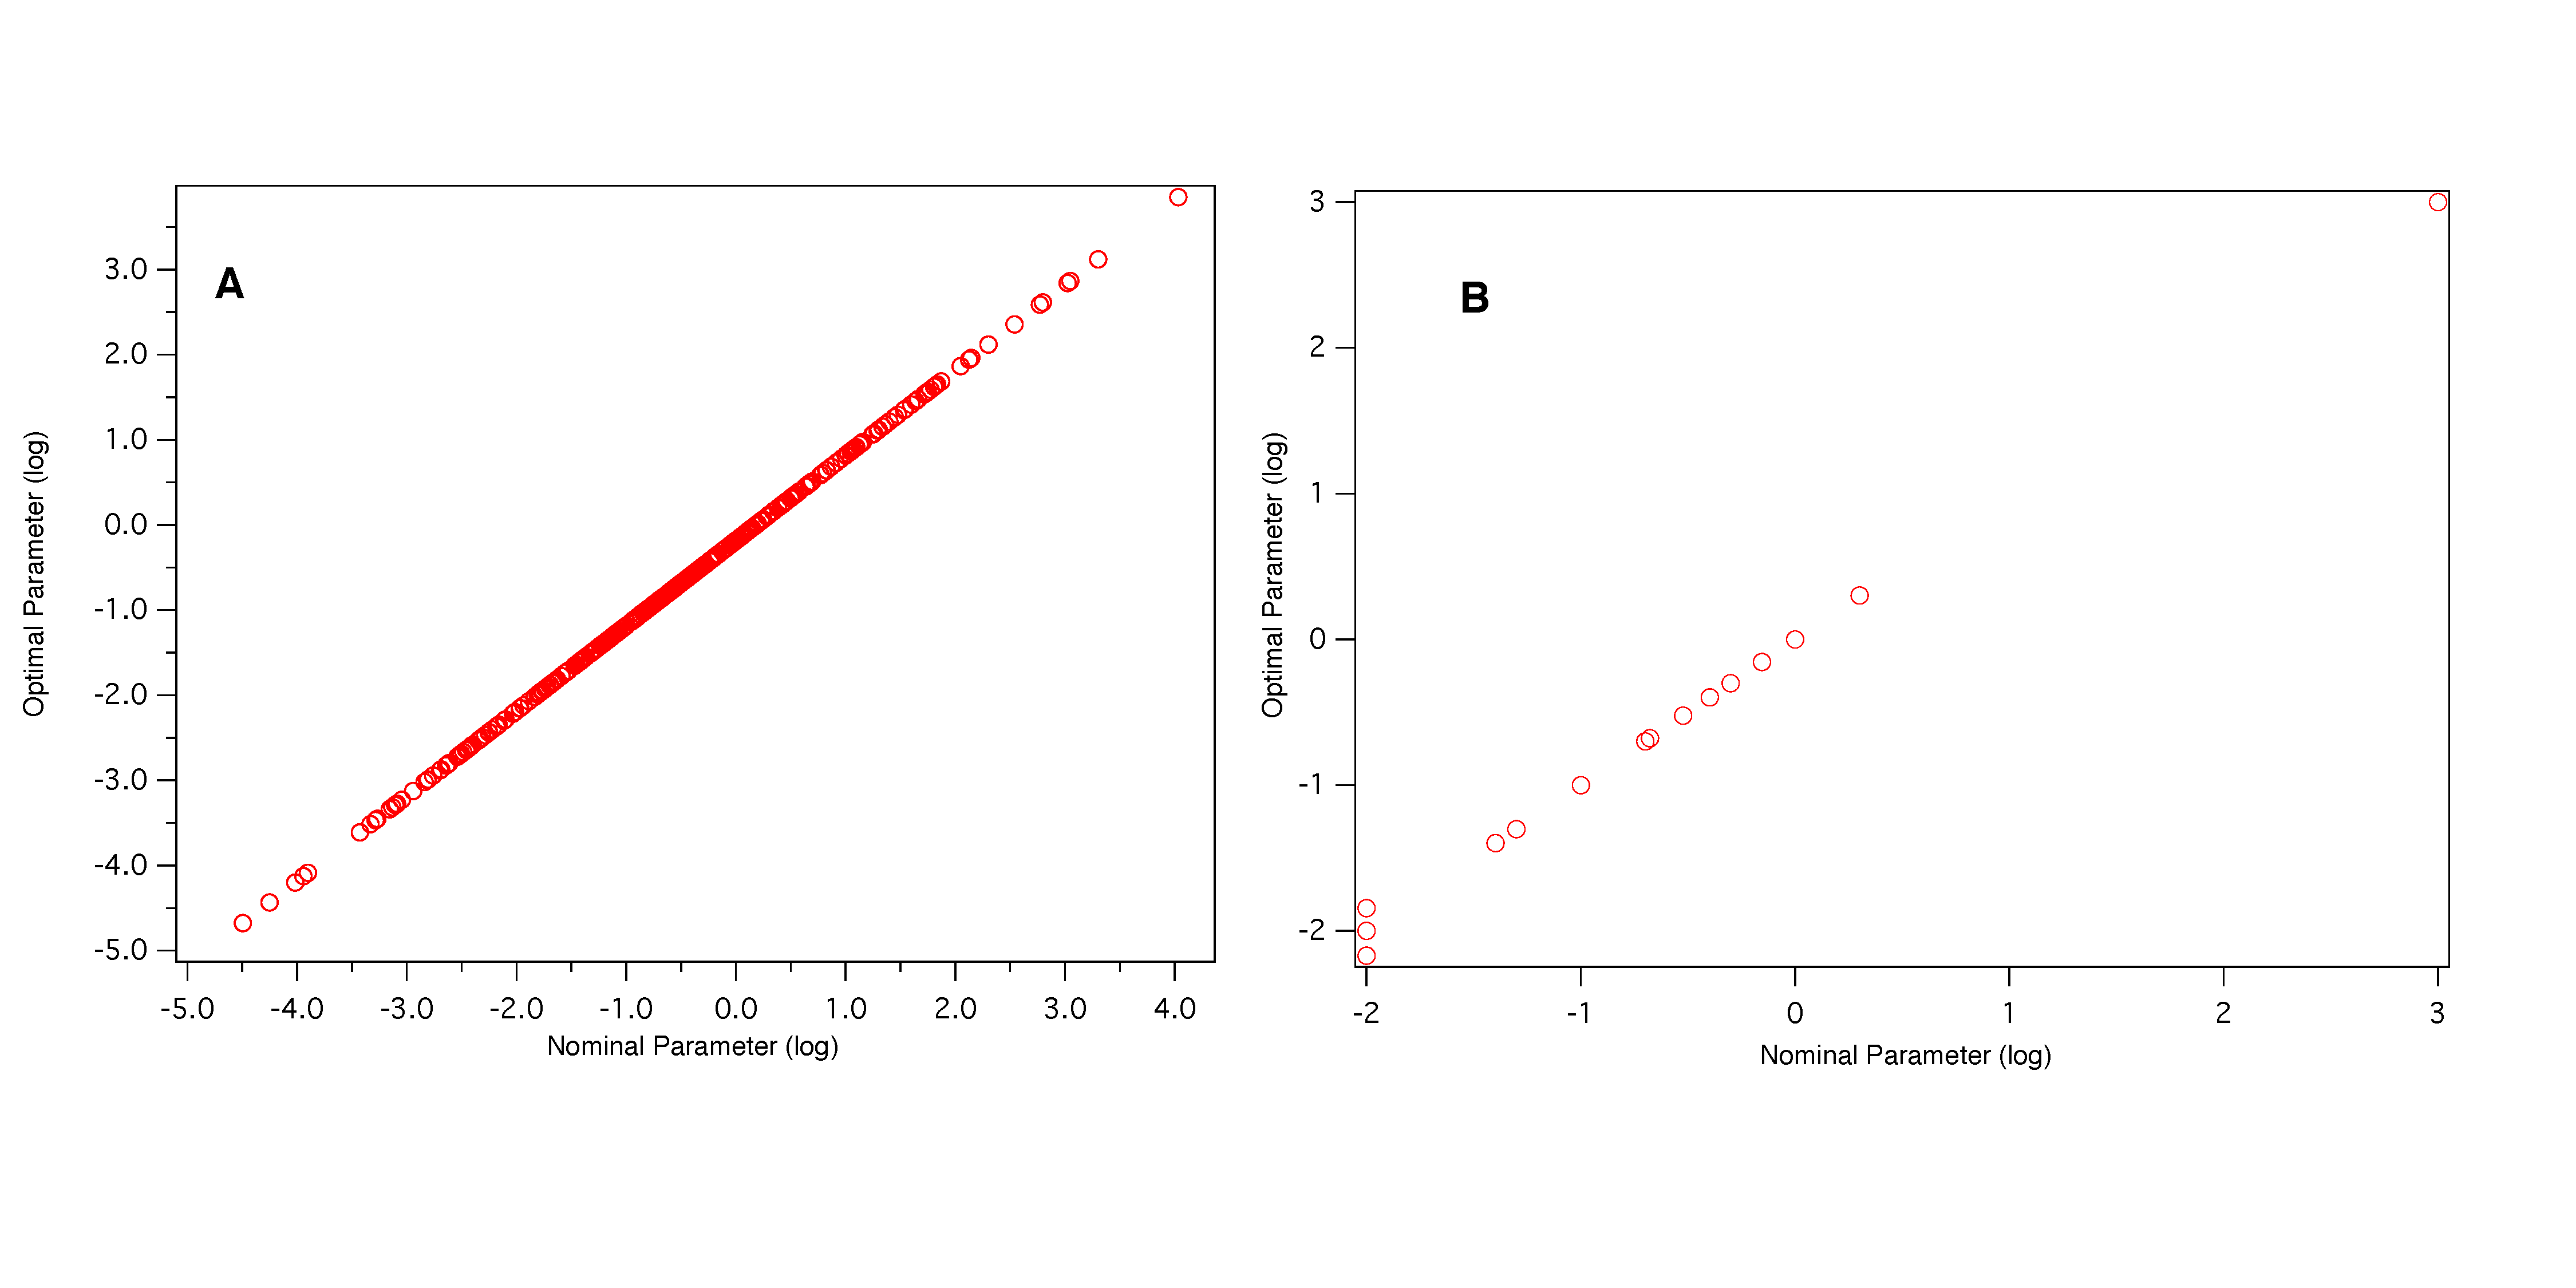
\includegraphics[width=1.02\textwidth,height=0.5\textheight]{./figs/Figure_7_Benchmarks_Parameters}
\caption{Difference between optimal and nominal parameter vector values on benchmark problems. \textbf {(A)} Problem B1: Genome wide kinetic model of E.coli \textit{S.cerevisiae} with 1759 unknown parameters. \textbf {(B)} Problem B4: Metabolic model of Chinese  Hamster Ovary Cells (CHO) cells with 117 parameters.
}\label{fig-benchmark}
\end{figure}




\end{document}
